% Options for packages loaded elsewhere
% Options for packages loaded elsewhere
\PassOptionsToPackage{unicode}{hyperref}
\PassOptionsToPackage{hyphens}{url}
%
\documentclass[
  hebrew,
  12pt,
  a4paper,
  oneside]{book}
\usepackage{xcolor}
\usepackage[right=30mm, left=30mm, top=30mm, bottom=30mm]{geometry}
\usepackage{amsmath,amssymb}
\setcounter{secnumdepth}{5}
\usepackage{iftex}
\ifPDFTeX
  \usepackage[T1]{fontenc}
  \usepackage[utf8]{inputenc}
  \usepackage{textcomp} % provide euro and other symbols
\else % if luatex or xetex
  \usepackage{unicode-math} % this also loads fontspec
  \defaultfontfeatures{Scale=MatchLowercase}
  \defaultfontfeatures[\rmfamily]{Ligatures=TeX,Scale=1}
\fi
\usepackage{lmodern}
\ifPDFTeX\else
  % xetex/luatex font selection
  \setmainfont[]{David}
  \setmonofont[]{Courier New}
\fi
% Use upquote if available, for straight quotes in verbatim environments
\IfFileExists{upquote.sty}{\usepackage{upquote}}{}
\IfFileExists{microtype.sty}{% use microtype if available
  \usepackage[]{microtype}
  \UseMicrotypeSet[protrusion]{basicmath} % disable protrusion for tt fonts
}{}
\usepackage{setspace}
\makeatletter
\@ifundefined{KOMAClassName}{% if non-KOMA class
  \IfFileExists{parskip.sty}{%
    \usepackage{parskip}
  }{% else
    \setlength{\parindent}{0pt}
    \setlength{\parskip}{6pt plus 2pt minus 1pt}}
}{% if KOMA class
  \KOMAoptions{parskip=half}}
\makeatother
% Make \paragraph and \subparagraph free-standing
\makeatletter
\ifx\paragraph\undefined\else
  \let\oldparagraph\paragraph
  \renewcommand{\paragraph}{
    \@ifstar
      \xxxParagraphStar
      \xxxParagraphNoStar
  }
  \newcommand{\xxxParagraphStar}[1]{\oldparagraph*{#1}\mbox{}}
  \newcommand{\xxxParagraphNoStar}[1]{\oldparagraph{#1}\mbox{}}
\fi
\ifx\subparagraph\undefined\else
  \let\oldsubparagraph\subparagraph
  \renewcommand{\subparagraph}{
    \@ifstar
      \xxxSubParagraphStar
      \xxxSubParagraphNoStar
  }
  \newcommand{\xxxSubParagraphStar}[1]{\oldsubparagraph*{#1}\mbox{}}
  \newcommand{\xxxSubParagraphNoStar}[1]{\oldsubparagraph{#1}\mbox{}}
\fi
\makeatother


\usepackage{longtable,booktabs,array}
\usepackage{calc} % for calculating minipage widths
% Correct order of tables after \paragraph or \subparagraph
\usepackage{etoolbox}
\makeatletter
\patchcmd\longtable{\par}{\if@noskipsec\mbox{}\fi\par}{}{}
\makeatother
% Allow footnotes in longtable head/foot
\IfFileExists{footnotehyper.sty}{\usepackage{footnotehyper}}{\usepackage{footnote}}
\makesavenoteenv{longtable}
\usepackage{graphicx}
\makeatletter
\newsavebox\pandoc@box
\newcommand*\pandocbounded[1]{% scales image to fit in text height/width
  \sbox\pandoc@box{#1}%
  \Gscale@div\@tempa{\textheight}{\dimexpr\ht\pandoc@box+\dp\pandoc@box\relax}%
  \Gscale@div\@tempb{\linewidth}{\wd\pandoc@box}%
  \ifdim\@tempb\p@<\@tempa\p@\let\@tempa\@tempb\fi% select the smaller of both
  \ifdim\@tempa\p@<\p@\scalebox{\@tempa}{\usebox\pandoc@box}%
  \else\usebox{\pandoc@box}%
  \fi%
}
% Set default figure placement to htbp
\def\fps@figure{htbp}
\makeatother

\ifLuaTeX
  \usepackage{luacolor}
  \usepackage[soul]{lua-ul}
\else
  \usepackage{soul}
\fi


\ifLuaTeX
\usepackage[bidi=basic,provide=*]{babel}
\else
\usepackage[bidi=default,provide=*]{babel}
\fi
\ifPDFTeX
\else
\babelfont{rm}[]{David}
\fi
% get rid of language-specific shorthands (see #6817):
\let\LanguageShortHands\languageshorthands
\def\languageshorthands#1{}


\setlength{\emergencystretch}{3em} % prevent overfull lines

\providecommand{\tightlist}{%
  \setlength{\itemsep}{0pt}\setlength{\parskip}{0pt}}



 


% pdf-env-boxes.tex — עטיפת סביבות LaTeX קיימות עם tcolorbox, מותאם לצבעי HTML
\usepackage{amsthm}
\usepackage[most]{tcolorbox}
\tcbuselibrary{theorems,skins,breakable,hooks}
\usepackage{xcolor}

% ==== שמות בעברית ====
\providecommand{\definitionname}{הגדרה}
\providecommand{\examplename}{דוגמה}
\providecommand{\exercisename}{תרגיל}
\providecommand{\remarkname}{הערה}
\providecommand{\theoremname}{משפט}
\providecommand{\lemmaname}{למה}
\providecommand{\propositionname}{טענה}
\providecommand{\corollaryname}{מסקנה}
\renewcommand{\proofname}{הוכחה}

% ==== צבעים (בהתאם ל-CSS: rgba) ====
\definecolor{envDefinitionRGB}{RGB}{255,99,71}    % tomato
\definecolor{envExampleRGB}{RGB}{138,43,226}      % blueviolet
\definecolor{envExerciseRGB}{RGB}{30,144,255}     % dodgerblue
\definecolor{envRemarkRGB}{RGB}{0,0,0}            % black (עם שקיפות נמוכה)
\definecolor{envTheoremRGB}{RGB}{255,165,0}       % orange
\definecolor{envProofRGB}{RGB}{60,179,113}        % mediumseagreen

% ==== סגנון בסיסי לכל התיבות ====
\tcbset{
  envbox/.style={
    enhanced, breakable, sharp corners,
    boxrule=0.4pt,
    colback=white,
    fonttitle=\bfseries\small,
    coltitle=black,
    title filled,
    left=8pt,right=8pt,top=6pt,bottom=6pt,
    before skip=10pt, after skip=10pt
  },
}

\makeatletter
% parent counter: ב-book לפי chapter, אחרת לפי section
\@ifundefined{c@chapter}{\def\qnumwithin{section}}{\def\qnumwithin{chapter}}

\newcommand{\EnsureNewTheorem}[2]{%
  \@ifundefined{#1}{%
    \newtheorem{#1}{#2}[\qnumwithin]%
  }{}%
}
\makeatother

\AtBeginDocument{%
  \theoremstyle{definition}
  \EnsureNewTheorem{definition}{\definitionname}
  \EnsureNewTheorem{example}{\examplename}
  \EnsureNewTheorem{exercise}{\exercisename}

  \theoremstyle{remark}
  \EnsureNewTheorem{remark}{\remarkname}

  \theoremstyle{plain}
  \EnsureNewTheorem{theorem}{\theoremname}
  \EnsureNewTheorem{lemma}{\lemmaname}
  \EnsureNewTheorem{proposition}{\propositionname}
  \EnsureNewTheorem{corollary}{\corollaryname}

  % ==== עטיפות עם צבעי HTML ====
  \tcolorboxenvironment{definition}{envbox,
    colframe=envDefinitionRGB,
    colbacktitle=envDefinitionRGB,
    colback=envDefinitionRGB!10,
    borderline south={0.4pt}{0pt}{envDefinitionRGB},
    title={\definitionname}}

  \tcolorboxenvironment{example}{envbox,
    colframe=envExampleRGB,
    colbacktitle=envExampleRGB,
    colback=envExampleRGB!10,
    borderline south={0.4pt}{0pt}{envExampleRGB},
    title={\examplename}}

  \tcolorboxenvironment{exercise}{envbox,
    colframe=envExerciseRGB,
    colbacktitle=envExerciseRGB,
    colback=envExerciseRGB!10,
    borderline south={0.4pt}{0pt}{envExerciseRGB},
    title={\exercisename}}

  \tcolorboxenvironment{remark}{envbox,
    colframe=envRemarkRGB,
    colbacktitle=envRemarkRGB,
    colback=envRemarkRGB!10,
    borderline south={0.4pt}{0pt}{envRemarkRGB},
    title={\remarkname}}

  \tcolorboxenvironment{theorem}{envbox,
    colframe=envTheoremRGB,
    colbacktitle=envTheoremRGB,
    colback=envTheoremRGB!10,
    borderline south={0.4pt}{0pt}{envTheoremRGB},
    title={\theoremname}}

  \tcolorboxenvironment{lemma}{envbox,
    colframe=envTheoremRGB,
    colbacktitle=envTheoremRGB,
    colback=envTheoremRGB!10,
    borderline south={0.4pt}{0pt}{envTheoremRGB},
    title={\lemmaname}}

  \tcolorboxenvironment{proposition}{envbox,
    colframe=envTheoremRGB,
    colbacktitle=envTheoremRGB,
    colback=envTheoremRGB!10,
    borderline south={0.4pt}{0pt}{envTheoremRGB},
    title={\propositionname}}

  \tcolorboxenvironment{corollary}{envbox,
    colframe=envTheoremRGB,
    colbacktitle=envTheoremRGB,
    colback=envTheoremRGB!10,
    borderline south={0.4pt}{0pt}{envTheoremRGB},
    title={\corollaryname}}

  \tcolorboxenvironment{proof}{envbox,
    colframe=envProofRGB,
    colbacktitle=envProofRGB,
    colback=envProofRGB!10,
    borderline south={0.4pt}{0pt}{envProofRGB},
    title={\proofname}}
}
\makeatletter
% מעטפת LTR למספרים
\newcommand{\LTRnum}[1]{\LR{#1}}

% תיקון תוכן העניינים: המספרים יוצגו LTR גם עם נקודות
\let\orig@numberline\numberline
\renewcommand{\numberline}[1]{\orig@numberline{\LTRnum{#1}}}

% סימניות ה-PDF (bookmarks) בלי פקודות כיווניות
\AtBeginDocument{%
  \@ifpackageloaded{hyperref}{%
    \pdfstringdefDisableCommands{\let\LTRnum\@firstofone}%
  }{}%
}
\makeatother
\usepackage{bidi}
\setRTL
% === I, II, III ואז 1, 2, ... ===
\usepackage{etoolbox}
\makeatletter
\setcounter{chapter}{0}% כך שהפרק הממוספר הראשון יהיה I
\newcounter{countedchap}
\pretocmd{\@chapter}{%
  \stepcounter{countedchap}%
  \ifnum\value{countedchap}=1
    \renewcommand{\thechapter}{\Roman{chapter}}%
  \fi
  % לאחר שלושה פרקים ברומי, הפרק הרביעי עובר לערבי ומתחיל מ-1
  \ifnum\value{countedchap}=4
    \renewcommand{\thechapter}{\arabic{chapter}}%
    \setcounter{chapter}{0}%
  \fi
}{}{}
\makeatother
\makeatletter
\@ifpackageloaded{bookmark}{}{\usepackage{bookmark}}
\makeatother
\makeatletter
\@ifpackageloaded{caption}{}{\usepackage{caption}}
\AtBeginDocument{%
\ifdefined\contentsname
  \renewcommand*\contentsname{תוכן עניינים}
\else
  \newcommand\contentsname{תוכן עניינים}
\fi
\ifdefined\listfigurename
  \renewcommand*\listfigurename{רשימת תרשימים}
\else
  \newcommand\listfigurename{רשימת תרשימים}
\fi
\ifdefined\listtablename
  \renewcommand*\listtablename{רשימת טבלאות}
\else
  \newcommand\listtablename{רשימת טבלאות}
\fi
\ifdefined\figurename
  \renewcommand*\figurename{תרשים}
\else
  \newcommand\figurename{תרשים}
\fi
\ifdefined\tablename
  \renewcommand*\tablename{טבלה}
\else
  \newcommand\tablename{טבלה}
\fi
}
\@ifpackageloaded{float}{}{\usepackage{float}}
\floatstyle{ruled}
\@ifundefined{c@chapter}{\newfloat{codelisting}{h}{lop}}{\newfloat{codelisting}{h}{lop}[chapter]}
\floatname{codelisting}{רישום}
\newcommand*\listoflistings{\listof{codelisting}{רשימת רישומים}}
\usepackage{amsthm}
\theoremstyle{remark}
\AtBeginDocument{\renewcommand*{\proofname}{הוכחה}}
\newtheorem*{remark}{הערה}
\newtheorem*{solution}{פתרון}
\newtheorem{refremark}{הערה}[chapter]
\newtheorem{refsolution}{פתרון}[chapter]
\makeatother
\makeatletter
\makeatother
\makeatletter
\@ifpackageloaded{caption}{}{\usepackage{caption}}
\@ifpackageloaded{subcaption}{}{\usepackage{subcaption}}
\makeatother
\usepackage{bookmark}
\IfFileExists{xurl.sty}{\usepackage{xurl}}{} % add URL line breaks if available
\urlstyle{same}
\hypersetup{
  pdftitle={אלגברה לינארית},
  pdfauthor={ד''ר יונתן שלח, ד''ר נדב מאיר},
  pdflang={he},
  hidelinks,
  pdfcreator={LaTeX via pandoc}}


\title{אלגברה לינארית}
\author{ד''ר יונתן שלח, ד''ר נדב מאיר}
\date{}
\begin{document}
\frontmatter
\maketitle

\renewcommand*\contentsname{תוכן עניינים}
{
\setcounter{tocdepth}{2}
\tableofcontents
}

\setstretch{1.5}
\mainmatter
\bookmarksetup{startatroot}

\chapter*{מידע כללי}\label{ux5deux5d9ux5d3ux5e2-ux5dbux5dcux5dcux5d9}
\addcontentsline{toc}{chapter}{מידע כללי}

\markboth{מידע כללי}{מידע כללי}

מבוא להנדסת תהליכים

ענבל צרפתי-ברנע

מיועד לסטודנטים וסטודנטיות בתחילת דרכם בלימודי הנדסת תהליכים

\subsubsection*{תודות}\label{ux5eaux5d5ux5d3ux5d5ux5ea}
\addcontentsline{toc}{subsubsection}{תודות}

ד״ר רחל ליכנשטיין, המחלקה להנדסת ביוטכנולוגיה על שם גולדה-מאיר\\
אבנר וסבלה גולדשטיין-יגורן\\
פרופ׳ רונית ביטון, המחלקה להנדסה כימית\\
היחידה לקידום איכות ההוראה והלמידה -- אוניברסיטת בן-גוריון בנגב

\phantomsection\label{download-box}
\href{אלגברה-לינארית.pdf}{להורדת הספר ב PDF}

\bookmarksetup{startatroot}

\chapter{הקדמה}\label{ux5d4ux5e7ux5d3ux5deux5d4}

אלגברה לינארית היא אחת מאבני היסוד של המתמטיקה המודרנית. בתור התחלה, היא
קשורה באופן הדוק לגיאומטריה של המישור וגם לגיאומטריה של המרחב. בחטיבת
הביניים לומדים על משוואה בנעלם אחד, וגם על מערכת של שתי משוואות בשני
נעלמים. למשל:

\[\begin{cases}
3x+2y=8\\
x+y=3
\end{cases}\]

יש יותר מדרך אחת לפתור מערכת כזו, כמו להכפיל את המשוואה השנייה ב-\(2\)
ואז להחסיר אותה מהמשוואה הראשונה. כך מקבלים \(x=2\) ולבסוף \(y=1\) עי
הצבה באחת המשוואות. מבחינה גיאומטרית, כל משוואה מייצגת קו ישר במישור,
ופתרון המערכת מוביל לנקודת החיתוך של שני הישרים.

\begin{center}
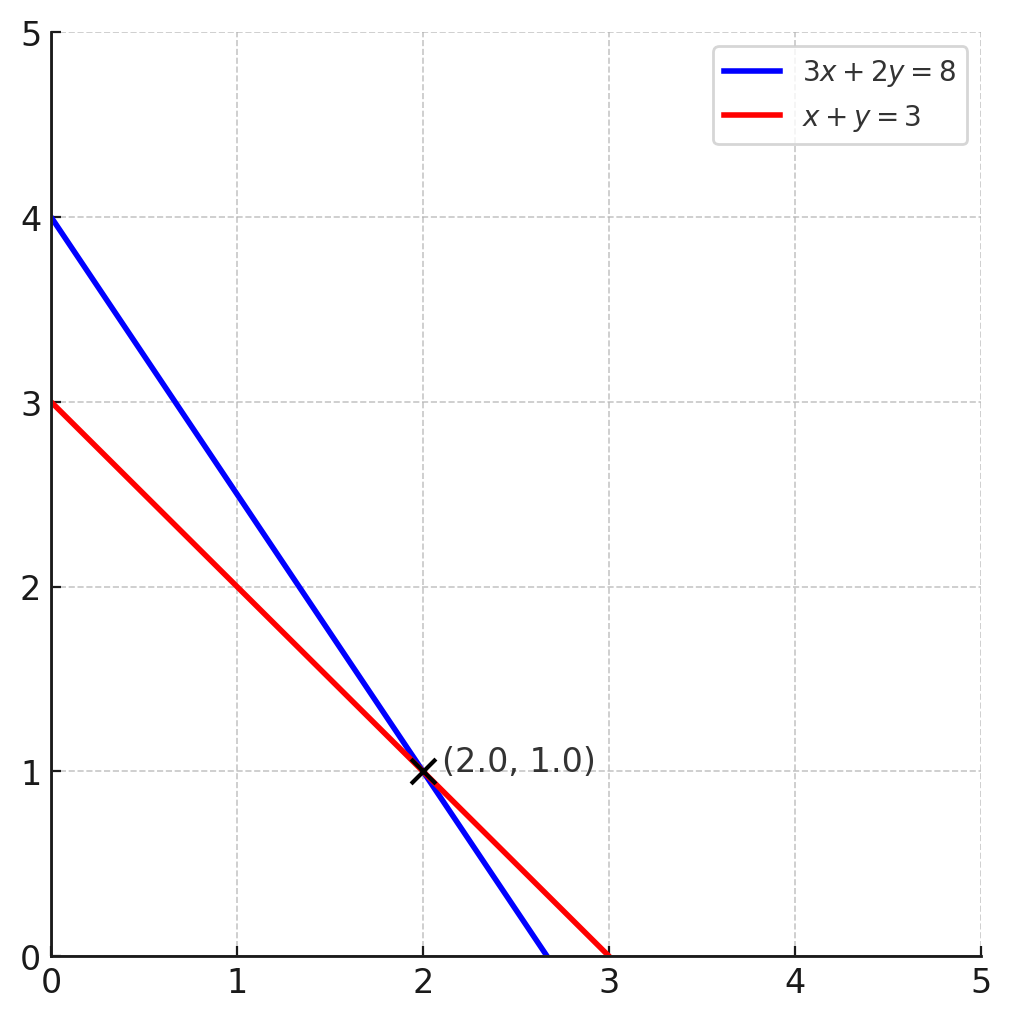
\includegraphics[width=0.5\linewidth,height=\textheight,keepaspectratio]{images/intro/intro_img_1.png}
\end{center}

איור 1: שני ישרים ונקודת החיתוך

בבסיסה אלגברה לינארית עוסקת בפתרון מערכת של משוואות לינאריות, כלומר
משוואות ממעלה ראשונה במספר נעלמים. בתחומים רבים במדע ובכלל יכולים להופיע
הרבה נעלמים והרבה (אילוצים) , בהתאם למה שידוע לנו על הבעיה הרלוונטית.

\begin{example}

תומר נוסע מאילת צפונה, ואלה נוסעת מתל אביב דרומה. המרחק ההתחלתי ביניהם
הוא \(350\) קמ. תומר נוסע במהירות \(60\) קמש במשך \(t_{1}\) שעות, וממשיך
במהירות \(90\) קמש במשך \(t_{2}\) שעות עד שהוא חולף על פני המכונית של
אלה ומזהה אותה. עד לרגע זה אלה נסעה במהירות \(90\) קמ במשך \(t_{3}\)
שעות ואחר כך במהירות \(110\) קמ במשך \(t_{4}\) שעות. אם נשווה בין סכומי
זמני התנועה של שתי המכוניות וגם נדרוש שסכום הדרכים יהיה המרחק ההתחלתי,
נקבל שתי משוואות בארבעה נעלמים:

\[\begin{cases}
t_{1}+t_{2}=t_{3}+t_{4}\\
60t_{1}+90t_{2}+90t_{3}+110t_{4}=350
\end{cases}\]

למערכת משוואות לינארית (ממל בראשי תיבות) זו יש אינסוף פתרונות בתחום
ההגדרה הרלוונטי של מספרים חיוביים. אם למשל נציב \(t_{3}=t_{4}=1\) בשתי
המשוואות, נקבל ממל חדשה של שתי משוואות בשני נעלמים:

\[\begin{cases}
t_{1}+t_{2}=2\\
60t_{1}+90t_{2}=150
\end{cases}\]

אפשר לפתור את הממל הזו כרגיל, אבל קל לבדוק שהפתרון הוא
\(t_{1}=t_{2}=1\). לכן, אחד הפתרונות של הממל המקורית (בארבעה נעלמים) הוא
\(t_{1}=t_{2}=t_{3}=t_{4}=1\). אבל זה לא הפתרון היחיד כי בחרנו את הערכים
של \(t_{3},t_{4}\) באופן שרירותי (נוח לחישובים, אך לא יותר מזה).

נראה בפרק איך אפשר לכתוב את קבוצת הפתרונות באופן כללי, אבל כבר אפשר
להבין שהיא אינסופית כי יש לנו חופש לבחור את ערכי \(t_{3},t_{4}\). אמנם
לא מדובר בחופש מוחלט כי כל ארבעת הזמנים צריכים להיות חיוביים (מה שמקטין
את קבוצת הפתרונות), אבל עדיין יש פה מספיק חופש לאינסוף פתרונות.

במובן מסוים אפשר לומר שאלה מחליטה בשביל תומר על זמני הנסיעה שלו. זו דרך
הסתכלות שרירותית ומאוד טכנית - אפשר לחשוב על פתרון המערכת גם באופן הפוך
ולתת את החופש לתומר. בפועל (מחוץ לעולם האלגברי) תומר ואלה לא שמו לב אחד
לשנייה עד לרגע הפגישה המקרית. להם יש מידע מלא על זמני הנסיעה, אבל אנחנו
מסתפקים במידע חלקי. אם היו לנו מספיק משוואות נוספות (לפחות שתיים), היה
ניתן להגיע לפתרון המדויק שמתאר את תנועת המכוניות. אבל לא תמיד יש לנו
מספיק מידע ונלמד להתייחס לכך בהתאם.

\end{example}

באופן כללי, נשאל את השאלות הבאות:

• כיצד פותרים ממל שבה הרבה נעלמים?

• כיצד פותרים ממל שבה הרבה משוואות?

• האם בכלל קיימים פתרונות לממל? אם כן, אז כמה?

כדי לענות על שאלות כאלו באופן מלא ומסודר, ישמשו אותנו שני מושגים
יסודיים: וקטורים ומטריצות. נדחה את ההגדרות שלהם לפרקים הרלוונטיים, אבל
לעת עתה מספיק לחשוב עליהם כאובייקטים מתמטיים שבהם מופיעים כמה מספרים.
למשל, הזוג הסדור \((x,y)\) של שני מספרים \(x\) ו-\(y\) הוא וקטור עם שני
רכיבים (קוארדינטות). בחטיבת הביניים ובתיכון ראינו שאפשר לחשוב על זוג כזה
כעל נקודה סטטית במישור, אבל בלימודי הפיזיקה יש הסתכלות דינמית על וקטור
כאובייקט בעל גודל וכיוון, לדוגמא כוח שפועל על גוף. נראה שאפשר לאמץ את
שתי הגישות (סטטית ודינמית) במקביל, כאשר האינטואיציה הפיזיקלית מועילה
מאוד אך ממש לא הכרחית להבנת הקורס.

לאחר שנתרגל לוקטורים ומטריצות, נראה שאפשר להסתכל עליהם באופן מופשט
(תיאורטי) ולשאול עליהם כל מיני שאלות שלא בהכרח קשורות לממל כזו או אחרת.
במתמטיקה, דבר אחד מוביל למשנהו וזה טוב לשמור על ראש פתוח כשלומדים מושגים
חדשים. הגישה המופשטת של אלגברה לינארית מאפשרת יישומים מגוונים, גם מחוץ
לגיאומטריה ופיזיקה. לטובת הסקרנים, נעסוק קצת בפיזיקה דרך הנדסה בחלק
מהיישומים בסוף הספר שחורגים מהקורס עצמו. אבל גם נעסוק ביישומים שקשורים
למאגר גדול של נתונים כמו למידת מכונה.

רבים מכם לומדים חשבון דיפרנציאלי ואינטגרלי במקביל. אפשר לומר שאלגברה
לינארית מופיעה בחשבון דיפרנציאלי ואינטגרלי הרבה יותר מאשר להיפך. מושג
הנגזרת מוביל לקירוב לינארי של פונקציה נתונה עי פונקציה לינארית שמתארת את
הישר המשיק לגרף הפונקציה בנקודה נתונה. בנוסף, הקשר לאלגברה לינארית מתבטא
בחישוב שטחים (במישור) ונפחים (במרחב) בעזרת כלי שנקרא דטרמיננטה. נפתח
אותו בפרק .

{[}תמונה - ישר משיק בצד אחד, מישור משיק בצד שני{]}

בספר מופיעות דוגמאות רבות, תרגילים פתורים וגם קישורים לסרטונים. תוכלו
לחזור אליו בהמשך התואר ככל שתצטרכו להשתמש באלגברה לינארית.

\bookmarksetup{startatroot}

\chapter{קבוצות
ומספרים}\label{ux5e7ux5d1ux5d5ux5e6ux5d5ux5ea-ux5d5ux5deux5e1ux5e4ux5e8ux5d9ux5dd}

\section{קבוצת המספרים הטבעיים והגדרת
קבוצה}\label{ux5e7ux5d1ux5d5ux5e6ux5ea-ux5d4ux5deux5e1ux5e4ux5e8ux5d9ux5dd-ux5d4ux5d8ux5d1ux5e2ux5d9ux5d9ux5dd-ux5d5ux5d4ux5d2ux5d3ux5e8ux5ea-ux5e7ux5d1ux5d5ux5e6ux5d4}

המתמטיקה מתחילה בחשבון, וחשבון מבוסס על ספירה. המספר \(1\) מתאר את
היחידה הבסיסית, (לצורך העניין אצבע אחת) שבעזרתה אפשר לספור כל מיני
דברים. ניתן להוסיף \(1\) לספירה כאוות נפשנו, ואם נמשיך כך, לנצח בדמיון
שלנו לפחות, נייצר אינסוף מספרים שלא בהכרח נדע איך לקרוא להם כי השמות
יהיו ארוכים מאוד. אבל יש שם לקבוצה של כל המספרים האלה: מספרים טבעיים.
הסימון המקובל הוא \(\mathbb{N}\), ואפשר למנות את איברי הקבוצה באופן הבא
\[\mathbb{N}=\{1,1+1,1+1+1,...\}=\{1,2,3,...\}\]

הסוגריים המסולסלים מתארים קבוצה שאיבריה מופיעים בין הסוגריים ומופרדים עי
פסיקים. מאחר שהקבוצה אינסופית, אנחנו נאלצים לכתוב ... מתוך הנחה שברור
איך להמשיך.

\begin{remark}
לפעמים גם \(0\) נחשב מספר טבעי, אבל לא בקורס שלנו וזה לא באמת חשוב.
מבחינה היסטורית ופילוסופית, \(0\) הוא מספר מוזר ומיוחד כי לא רואים אותו
בטבע. הוא מתאר את מה שאינו.
\end{remark}

\begin{definition}

קבוצה היא אוסף כלשהו של איברים (לא בהכרח מספרים) ללא חשיבות לסדר הופעתם.

\end{definition}

זו הגדרה מאוד כללית, ובלבד שיהיה ברור מהגדרת הקבוצה אילו איברים שייכים
לה ואילו לא. אם הקבוצה היא \(A\), אז נכתוב \(a\in A\) כדי לומר שהאיבר
\(a\) שייך לקבוצה \(A\). אם הוא לא שייך לה, נכתוב \(a\notin A\).

עיגול עם נקודה בתוכו שמסומנת כשייכת, ונקודה בחוץ שמסומנת כלא שייכת

\begin{example}

משפחת לוי כוללת את דרור , אורית ואיתי. נקרא לקבוצת אנשים זו \(L\) ונתאר
אותה באופן מפורש תוך שימוש בלועזית (אפשר גם בעברית)
\[L=\{\text{{Dror, Itay, Orit}}\}\]

בפרט, מתקיים \(Itay \in L\) אך \(Ofer \notin L\) כי מבין השניים האלה רק
איתי שייך למשפחה. נדגיש שאין חשיבות לסדר האיברים בתוך הקבוצה, ובדרך כלל
יש יותר מדרך אחת להציג את הקבוצה. למשל, כאן גם מתקיים
\[L=\{\text{{Itay, Dror, Orit}}\}=\{\text{{Orit, Itay, Dror}}\}\]

\end{example}

\begin{exercise}

האם מתקיים \(100^{100}\in\mathbb{N}\)? \(100^{-100}\in\mathbb{N}\)?
\((-100)^{100}\in\mathbb{N}\)?

\end{exercise}

ניתן להגדיר תת-קבוצות של \(\mathbb{N}\) עי שימוש בתכונות. למשל, את קבוצת
המספרים הזוגיים החיוביים \(2\mathbb{N}\) ניתן להגדיר באופן הבא:
\[2\mathbb{N}=\{n\in\mathbb{N}|n\text{ {is divided by} 2}\}=\{2,4,6,...\}\]

הסימן \(\in\) מתאר שייכות, ולכן הנוסחה \(n\in\mathbb{N}\) פירושה המספר
\(n\) שייך לקבוצה \(\mathbb{N}\). הקו \(|\) שמפריד בין הנוסחה לתנאי,
פירושו כך ש-. לכן, הגדרת הקבוצה אומרת לנו שמדובר בקבוצת כל המספרים
מהצורה \(n\in\mathbb{N}\) כך ש-\(n\) מתחלק ב-\(2\). אפשר גם להגדיר את
הקבוצה הזו עי נוסחה מפורשת \(2n\) שתפיק את כל המספרים הזוגיים החיוביים
כאשר נציב בה כל מספר מהצורה \(n\in\mathbb{N}\). הפעם הכתיבה היא כדלקמן
\[2\mathbb{N}=\{2n|n\in\mathbb{N}\}\]

שימו לב ששתי צורות הכתיבה דומות נוסחה בצד שמאל ותנאי בצד ימין, עם קו
מפריד באמצע. ההבדל הוא שבצורה הראשונה הנוסחה מתייחסת לקבוצה ידועה
\(\mathbb{N}\), והתנאי דרוש כדי לקבוע את השייכות לקבוצה החדשה. בצורה
השנייה יש נוסחה של משתנה \(n\), והתנאי מתייחס לערכי המשתנה שיש להציב
בנוסחה כאן התנאי הוא זה שמתייחס ל-\(\mathbb{N}\). בהמשך הפרק נוכיח שאכן
שתי ההגדרות של קבוצת הזוגיים הן הגדרות שקולות, כלומר שתיהן אכן מתארות את
המספרים \(2,4,6,...\) ושום מספר אחר. זה אולי כבר נראה ברור, אבל נשאלת
השאלה איך כותבים הוכחה מסודרת.

\section{קבוצות מספרים
נוספות}\label{ux5e7ux5d1ux5d5ux5e6ux5d5ux5ea-ux5deux5e1ux5e4ux5e8ux5d9ux5dd-ux5e0ux5d5ux5e1ux5e4ux5d5ux5ea}

ב-\(\mathbb{N}\) יש פעולות חיבור וכפל. הפעולות ההפוכות, חיסור וחילוק,
דורשות הרחבה של \(\mathbb{N}\) לקבוצות יותר גדולות. למשל, למשוואה
\(x+2=1\) אין פתרון טבעי ואנחנו יודעים שאפשר לפתור אותה עי חיסור \(2\)
מכל אגף ואז הפתרון יהיה \(x=-1\), שהוא מספר שלילי. בעצם, מגדירים את
\(-1\) כפתרון של המשוואה \(x+1=0\) וזה מוביל להגדרה של המספרים השלמים
\[\mathbb{Z}=\{...,-3,-2,-1,0,1,2,3,...\}=\{n-m|n,m\in\mathbb{\mathbb{N}}\}\]

שימו לב לכתיבה בצד ימין. זו דרך להגדיר את קבוצת השלמים בעזרת קבוצת
הטבעיים, כאשר הכוונה היא לקבוצת כל המספרים מהצורה \(n-m\) כאשר \(n,m\)
הם מספרים טבעיים. יש יותר מדרך אחת לכתוב מספר שלם כהפרש של מספרים טבעיים
(למעשה אינסוף).

ניתן גם להרחיב את \(\mathbb{Z}\) כך שיהיה ניתן לבצע חילוק. בתור התחלה
מגדירים לכל \(m\neq0\) שלם את המספר ההופכי \(\frac{1}{m}\), וכדי לאפשר
כפל גם מוסיפים את כל השברים מהצורה \(\frac{n}{m}\) כאשר
\(n\in\mathbb{Z}\). כך מקבלים את קבוצת המספרים הרציונליים
\[\mathbb{Q}=\{\frac{n}{m}|m,n\in\mathbb{\mathbb{Z}},\,m\neq0\}\]

גם כאן יש אינסוף דרכים להציג מספר רציונלי כמנה של מספרים שלמים, ואין עם
זה בעיה מבחינת הגדרת הקבוצה. אנחנו רגילים להצגה הפשוטה ביותר, לאחר צמצום
המחלקים המשותפים של המונה והמכנה.

זה מביא אותנו לקבוצת המספרים הממשיים \(\mathbb{R}\), שהיא הקבוצה העיקרית
שנתמקד בה בקורס. קבוצה זו מכילה את קבוצת המספרים הרציונליים (כל מספר
רציונלי הוא ממשי(, אבל יש בה מספרים נוספים שנקראים אי-רציונליים. יש הרבה
מה לומר על מספרים ממשיים, אבל הדיון המלא מתאים לקורס בחשבון דיפרנציאלי
ואינטגרלי. אז נסתפק באפיון הבא: ניתן להציג כל \(x\in\mathbb{R}\) בהצגה
עשרונית מהצורה \[x=\pm d_{n}...d_{2}d_{1}d_{0}.d_{-1}d_{-2}d_{-3}...\]
כאשר \(d_{n},d_{n-1},...,d_{0},d_{-1},d_{-2},...\) הן ספרות עשרוניות בין
\(0\) ל-\(9\) (כולל(, והנקודה העשרונית מפרידה בין החלק השלם משמאל לחלק
השברי מימין. \(x\) הוא רציונלי כאשר סדרת הספרות העשרוניות היא מחזורית
החל משלב מסוים. למשל

\[\begin{aligned}
\frac{1}{5}=0.200000000000...\\
\frac{1}{6}=0.166666666666...\\
\frac{1}{7}=0.142857142857...
\end{aligned}\]

במקרה הראשון הספרה \(0\) חוזרת על עצמה (אפשר להשמיט אותה ולקבל הצגה
סופית(, במקרה השני הספרה \(6\) חוזרת על עצמה, ובמקרה השלישי הרצף
\(142857\) חוזר על עצמו. המחזוריות נובעת מאופן החישוב של הספרות
העשרוניות (לפי חילוק ארוך(.

המספר הוא אי-רציונלי כאשר אין מחזוריות באף שלב של ההצגה העשרונית, ואז
החוקיות של סדרת הספרות העשרוניות עלולה להיות מסובכת מאוד. למשל
\[\begin{aligned}
\sqrt{2}=1.41421356237309504880168872420969807856967187537...\\
\pi=3.14159265358979323846264338327950288419716939937...
\end{aligned}\] נדגיש שאלה מספרים אי-רציונליים מיוחדים כי יש להם משמעות
גיאומטרית. \(\sqrt{2}\) הוא אורך היתר של משולש ישר-זווית עם שני ניצבים
באורך \(1\), לפי משפט פיתגורס. \(\pi\) הוא היקף מעגל שקוטרו באורך \(1\).

מבחינת הקורס, המספרים האי-רציונליים הרלוונטיים הם בעיקר שורשים כמו
\(\sqrt{2}\) שהם יחסית נוחים לחישובים. אבל טוב לזכור שיש המון מספרים
אי-רציונליים (יותר מאשר מספרים רציונליים במובן מסוים(, והם משלימים את
המספרים הרציונליים למה שנקרא הישר הממשי. ניתן לחשוב על המספרים כנקודות
על ישר עם ראשית \(0\). המספרים החיוביים מופיעים בצד ימין, ואילו המספרים
השליליים מופיעים בצד שמאל.

(הישר הממשי(

נשארה עוד קבוצה אחת, שהיא הגדולה ביותר מבין קבוצות המספרים שנעסוק בהן.
באופן דומה להגדרת \(-1\) כשורש (פתרון( של המשוואה \(x+1=0\), אפשר להגדיר
את \(i\) כשורש של המשוואה \(x^{2}+1=0\). זהו מספר מדומה, שהרי אין פתרון
ממשי למשוואה זו (ערך המינימום של הפונקציה הוא \(1\)(. המספר \(i\) לא
ניתן למדידה במציאות אך הוא שימושי מאוד במתמטיקה, פיזיקה וחלק מההנדסות.
לפי ההגדרה מתקיים \(i^{2}=-1\) וזה מספיק כדי להגדיר את קבוצת המספרים
המרוכבים ואת פעולות החשבון המתאימות לה.

\[\mathbb{\mathbb{C}}=\{a+bi|a,b\in\mathbb{R}\}\]

ההצגה \(a+bi\) עבור \(a,b\in\mathbb{R}\) הינה יחידה. כלומר, אם מתקיים
\(a+bi=c+di\) עבור \(c,d\in\mathbb{R}\), אז בהכרח \(a=c,\,b=d\).

עבור \(z=x+yi\) מרוכב עם \(x,y\in\mathbb{R}\) נגדיר את החלק הממשי
\(\text{{Re}}(z)=x\) ואת החלק המדומה \(\text{{Im}}(z)=y\). בנוסף, נגדיר
את המספר הצמוד \(\overline{z}=x-yi\).

שימו לב כי בניגוד לשמו, החלק המדומה הוא מספר ממשי זהו המקדם של \(i\),
שהוא עצמו באמת מדומה. מספר מרוכב נקרא מדומה אם החלק הממשי שלו הוא \(0\),
(כלומר זה מספר מהצורה \(yi\) כאשר \(y\in\mathbb{R}\))

א. \(\text{{Re}}(3+5i)=3,\:\text{{Im}}(3+5i)=5,\:\overline{3+5i}=3-5i\)

ב. \(\text{{Re}}(4i)=0,\:\text{{Im}}(4i)=4,\:\overline{4i}=-4i\)

ג. \(\text{{Re}}(3)=3,\:\text{{Im}}(3)=0,\:\overline{3}=3\) כאשר זיהינו
את \(3\) כמספר מרוכב עם חלק מדומה \(0\) לפי ההצגה \(3=3+0\cdot i\).

\begin{exercise}

לכל \(z\in\mathbb{C}\) הראו כי המספר הצמוד ל-\(\overline{z}\) הוא \(z\).

\end{exercise}

בפרק הבא נדון בפעולות, תכונות וחלק מהשימושים של המספרים המרוכבים. את סוף
הפרק הזה נקדיש לקשר בין כל קבוצות המספרים.

\section{תורת הקבוצות על קצה
המזלג}\label{ux5eaux5d5ux5e8ux5ea-ux5d4ux5e7ux5d1ux5d5ux5e6ux5d5ux5ea-ux5e2ux5dc-ux5e7ux5e6ux5d4-ux5d4ux5deux5d6ux5dcux5d2}

ראינו את יחס השייכות בין איבר \(a\) לקבוצה \(A\), וסימנו \(a\in A\).
בקורס שלנו הקבוצות יהיו יחסית פשוטות, ולכן לא ניתקל בקבוצה שאיבריה הם גם
קבוצות. זה בהחלט תרחיש אפשרי במתמטיקה (למשל קבוצה של שני ישרים, כאשר כל
ישר הוא קבוצת נקודות(, אבל בקורס נעסוק בקבוצות מספרים וקבוצות וקטורים
(וקטורים אינם קבוצות(. בכל אופן, ייתכן קשר יותר טבעי בין שתי קבוצות
\(A,B\).

\begin{definition}

נאמר ש-\(A\) מוכלת ב-\(B\) ונסמן \(A\subseteq B\) אם כל איבר של \(A\)
הוא גם איבר של \(B\).

באופן קצת יותר מתמטי \(A\subseteq B\) אם לכל \(a\in A\) מתקיים
\(a\in B\).

אם ההיפך הוא הנכון, כלומר קיים \(a\in A\) עבורו \(a\notin B\), אז נסמן
\(A\nsubseteq B\) ונאמר ש-\(A\) לא מוכלת ב-\(B\).

\end{definition}

(עיגול בתוך עיגול כדי לתאר הכלה, ושני עיגולים שרק נחתכים כדי לתאר חוסר
הכלה(

\begin{example}

עבור \(A=\{1,2\},\,B=\{1,2,3\}\) מתקיים \(A\subseteq B\) כי גם
\(1\in B\) וגם \(2\in B\). אבל \(B\nsubseteq A\) כי \(3\in B\) אך
\(3\notin A\).

\end{example}

נגדיר \(A=\{1,3\},\,B=\{-1,1,2,3\},\,C=\{-1,2\}\). מצאו את כל זוגות
הקבוצות שמקיימות קשר של הכלה.

\begin{definition}

נאמר ששתי קבוצות \(A,B\) הן שוות ונסמן \(A=B\) אם יש בהן בדיוק אותם
האיברים, כלומר מתקיים \(x\in A\) אם ורק אם \(x\in B\).

\end{definition}

\begin{remark}
כדי להוכיח כי \(A=B\), הדרך המקובלת היא להוכיח כי \(A\subseteq B\) וגם
\(B\subseteq A\). דרך הוכחה זו נקראת הכלה דו-צדדית.
\end{remark}

נסכם את רעיון ההוכחה: מוכיחים שתי הכלות. לכל הכלה מתחילים את הטיעון ביהי
כדי להצהיר שבחרנו איבר כללי מתוך הקבוצה הנתונה. אחר כך משתמשים בהגדרת
הקבוצה כדי להראות שהאיבר גם מקיים את ההגדרה של הקבוצה השנייה.

\begin{proposition}

\(\mathbb{N\subseteq\mathbb{Z}\subseteq\mathbb{Q}\subseteq\mathbb{R}\subseteq\mathbb{\mathbb{C}}}\)
וכל הקבוצות שונות זו מזו.

\end{proposition}

\begin{proof}
ברור כי \(\mathbb{N}\subseteq\mathbb{Z}\) לפי הגדרת \(\mathbb{Z}\)
כהרחבה של \(\mathbb{N}\), ורואים שאין שוויון כי \(-1\notin\mathbb{N}\).
גם דיברנו על ההכלה \(\mathbb{Q}\subseteq\mathbb{R}\) שאינה שוויון, כי
המספרים הרציונליים הם בדיוק המספרים הממשיים שיש להם הצגה עשרונית שהיא
מחזורית החל ממקום מסוים. יש הרבה מספרים ממשיים שאינם כאלה, למשל
\(\sqrt{2}\notin\mathbb{Q}\).

נוכיח כי \(\mathbb{Z}\subseteq\mathbb{Q}\) יהי \(n\in\mathbb{Z}\).
מתקיים \(n=\frac{n}{1}\) וזו מנה של מספרים שלמים, ולכן
\(n\in\mathbb{Q}\). אז \(\mathbb{Z}\subseteq\mathbb{Q}\), ואין שוויון כי
למשל \(\frac{1}{2}\in\mathbb{Q}\) אך \(\frac{1}{2}\notin\mathbb{Z}\).

נוכיח כי \(\mathbb{\mathbb{R}}\subseteq\mathbb{\mathbb{C}}\) יהי
\(x\in\mathbb{\mathbb{R}}\). מתקיים \(x=x+0\cdot i\) וזו הצגה של מספר
מרוכב, ולכן \(x\in\mathbb{C}\). אז
\(\mathbb{\mathbb{R}}\subseteq\mathbb{\mathbb{C}}\), ואין שוויון כי למשל
\(i\in\mathbb{C}\) אך \(i\notin\mathbb{\mathbb{R}}\).
\end{proof}

\section{פעולות בין
קבוצות}\label{ux5e4ux5e2ux5d5ux5dcux5d5ux5ea-ux5d1ux5d9ux5df-ux5e7ux5d1ux5d5ux5e6ux5d5ux5ea}

\begin{definition}

בהינתן שתי קבוצות \(A,B\) נגדיר את הקבוצות הבאות

א. החיתוך \(A\cap B\) הוא קבוצת כל האיברים השייכים גם ל-\(A\) וגם
ל-\(B\).

ב. האיחוד \(A\cup B\) הוא קבוצת כל האיברים השייכים לפחות לאחת משתי
הקבוצות \(A,B\).

\end{definition}

(דיאגרמות ון לשתי קבוצות האחת לחיתוך, השנייה לאיחוד עם צבע שונה(

\begin{remark}
במקרה של איחוד זה לא משנה אם האיבר שייך רק לקבוצה אחת או לשתיהן. בכל
מקרה הוא נספר רק פעם אחת באיחוד.
\end{remark}

\begin{example}

א. עבור \(A=\{1,2,3\},\,B=\{2,3,4\}\) מתקיים
\[.A\cap B=\{2,3\},\,A\cup B=\{1,2,3,4\}\]

ב. מתקיים
\(\mathbb{R}\cap\mathbb{C}=\mathbb{R},\,\mathbb{R}\cup\mathbb{C}=\mathbb{C}\)
כי \(\mathbb{R\subseteq\mathbb{C}}\).

ג. נסמן
\(D = \{\, n \in \mathbb{N} \mid 5 \mid n \,\}, \quad C = \{\, n \in \mathbb{N} \mid 3 \mid n \,\}\)
\textbackslash{} אז לפי הגדרת החיתוך והעובדה ש-\(3,5\) הם מספרים זרים
(המחלק המשותף היחיד שלהם הוא \(1\)), נובע כי
\[ C \cap D = \{\, n \in \mathbb{N} \mid 3 \mid n \ \land\ 5 \mid n \,\} = \{\, n \in \mathbb{N} \mid 15 \mid n \,\} \\ = \{15,30,45,\ldots\} \]

האפיון של האיחוד פחות פשוט: מדובר בקבוצת כל המספרים שמתחלקים ב-\(3\),
\(5\) או בשניהם (כלומר ב-\(15\), המקרה של החיתוך(. כך נקבל
\[.C\cup D=\{3,5,6,9,10,12,15,18,20,21,24,25,27,30...\}\]

\end{example}

חשבו את \(A\cap B,\,A\cup B\) עבור \(A=\{-1,0,1\},\,B=\{-2,0,1,2\}\).

\begin{proposition}

לכל שתי קבוצות \(A,B\) מתקיים \[.A\cap B\subseteq A\subseteq A\cup B\]

\end{proposition}

\begin{proof}
יש כאן שתי הכלות. נוכיח תחילה כי \(A\cap B\subseteq A\) יהי
\(a\in A\cap B\). אז מיידית לפי הגדרת החיתוך מתקיים \(a\in A\) ולכן
\(A\cap B\subseteq A\).

כעת נוכיח כי \(A\subseteq A\cup B\). גם כאן זה מיידי כי כל \(x\in A\)
מקיים את הגדרת האיחוד (בין אם \(x\in B\) ובין אם לאו(.
\end{proof}

\begin{remark}
באותו אופן (או משיקולי סימטריה) גם מתקיים
\[.A\cap B\subseteq B\subseteq A\cup B\]
\end{remark}

\section*{תרגילים}\label{ux5eaux5e8ux5d2ux5d9ux5dcux5d9ux5dd}
\addcontentsline{toc}{section}{תרגילים}

\markright{תרגילים}

הוכיחו כי \[.\{2n-1|n\in\mathbb{Z}\}=\{2m+1|m\in\mathbb{Z}\}\] הוכיחו כי
\[.\{z\in\mathbb{C}|\text{{Im}}(z)=2\text{{Re}}(z)\}=\{t+2ti|t\in\mathbb{R}\}\]

נגדיר \(A=\{\frac{1}{n}|n\in\mathbb{Z},\,n\neq0\}\).

א. חשבו את \(A\cap\mathbb{Z}\).

ב. הראו כי \(A\cup\mathbb{Z\subseteq\mathbb{\mathbb{Q}}}\), אך אין
שוויון.

\bookmarksetup{startatroot}

\chapter{המספרים
המרוכבים}\label{ux5d4ux5deux5e1ux5e4ux5e8ux5d9ux5dd-ux5d4ux5deux5e8ux5d5ux5dbux5d1ux5d9ux5dd}

\section{פעולות
חשבון}\label{ux5e4ux5e2ux5d5ux5dcux5d5ux5ea-ux5d7ux5e9ux5d1ux5d5ux5df}

נסמן \(z_{1}=a+bi,\,z_{2}=c+di\). נרחיב את הגדרות פעולות החשבון המוכרות
ל-\(\mathbb{C}\)

חיבור \(z_{1}+z_{2}=a+c+(b+d)i\)

חיסור \(z_{1}-z_{2}=a-c+(b-d)i\)

כפל \(z_{1}z_{2}=ac-bd+(ad+bc)i\)

חילוק
\(\frac{z_{1}}{z_{2}}=\frac{(a+bi)(c-di)}{(c+di)(c-di)}=\frac{ac+bd}{c^{2}+d^{2}}+\frac{(bc-ad)}{c^{2}+d^{2}}i\)
עבור \(z_{2}\neq0\).

הכפל מתאים לפתיחת סוגריים לפי חוקי הפילוג והחילוף של מספרים ממשיים.
בשביל חילוק מכפילים ומחלקים במספר הצמוד \(\overline{z_{2}}=c-di\) כדי
המכנה החדש יהיה מספר ממשי.

\begin{example}

ניקח \(z_{1}=1+i,\,z_{2}=2+3i\). כאן נקבל

חיבור \(z_{1}+z_{2}=3+4i\)

חיסור \(z_{1}-z_{2}=-1-2i\)

כפל \(z_{1}z_{2}=(1+i)(2+3i)=2-3+(3+2)i=-1+5i\)

חילוק
\(\frac{1+\text{i}}{2+3i}=\frac{(1+i)(2-3i)}{(2+3i)(2-3i)}=\frac{5}{13}-\frac{1}{13}i\)

\end{example}

\begin{exercise}

חשבו את ארבע הפעולות עבור \(z_{1}=1+2i,\,z_{2}=3-4i\).

\end{exercise}

\begin{remark}
נראה בהמשך שחיבור של מספרים מרוכבים שקול לחיבור בין שני וקטורים במישור,
ואכן ניתן לייצג כל מספר מרוכב \(z=x+yi\) כנקודה/וקטור במישור עם
קוארדינטות \((x,y)\). קוארדינטות אלו נקראות קרטזיות.
\end{remark}

\begin{proof}
לכל \(z_{1},z_{2},z_{3}\in\mathbb{C}\) מתקיים

א. חוקי החילוף לחיבור וכפל \(z_{1}+z_{2}=z_{2}+z_{1}\) וגם
\(z_{1}z_{2}=z_{2}z_{1}\).

ב. חוקי הקיבוץ לחיבור וכפל \((z_{1}+z_{2})+z_{3}=z_{1}+(z_{2}+z_{3})\)
וגם \((z_{1}z_{2})z_{3}=z_{1}(z_{2}z_{3})\).

ג. חוק הפילוג \((z_{1}+z_{2})z_{3}=z_{1}z_{3}+z_{2}z_{3}\)

ד. נייטרלי ביחס לחיבור \(z+0=z\) לכל \(z\in\mathbb{C}\).

ה. נייטרלי ביחס לכפל \(z\cdot1=z\) לכל \(z\in\mathbb{C}\).
\end{proof}

\begin{proof}
ישירות מן ההגדרות של חיבור וכפל תוך שימוש בחוקים המוכרים למספרים ממשיים.
נסתפק בהוכחת חוק החילוף לכפל ראשית נסמן \(z_{1}=a+bi,\,z_{2}=c+di\). לפי
הגדרת הכפל מתקיים \[.\begin{cases}
z_{1}z_{2}=(a+bi)(c+di)=ac-bd+(ad+bc)i\\
z_{2}z_{1}=(c+di)(a+bi)=ca-db+(cb+da)i
\end{cases}\]

נזכור כי \(a,b,c,d\in\mathbb{R}\) ולכן כבר ידוע שחוק החילוף תקף לגביהם
)גם לכפל וגם לחיבור(. לכן \(ac=ca,\,bd=db,\,ad=da,\,bc=cb\) ומכאן נובע
כי \(z_{1}z_{2}=z_{2}z_{1}\).
\end{proof}

נסכם את רעיון ההוכחה: השתמשנו בנוסחה של פעולת הכפל כדי להבין כיצד חוק
החילוף לכפל של מספרים מרוכבים, נובע מחוק החילוף המוכר לכפל של מספרים
ממשיים.

\begin{exercise}

הוכיחו את חוק החילוף לחיבור של מספרים מרוכבים.

\end{exercise}

הטענות הבאות קשורות להגדרה של מספר צמוד.

\begin{proof}
לכל \(z_{1},z_{2}\in\mathbb{C}\) מתקיים

א. \(\overline{z_{1}+z_{2}}=\overline{z_{1}}+\overline{z_{2}}\)

ב. \(\overline{z_{1}z_{2}}=\overline{z_{1}}\cdot\overline{z_{2}}\)
\end{proof}

\begin{proof}
נסמן \(z_{1}=a+bi,\,z_{2}=c+di\). נחשב

א.
\(\overline{z_{1}+z_{2}}=\overline{a+c+(b+d)i}=a+c-(b+d)i=a-bi+c-di=\overline{z_{1}}+\overline{z_{2}}\)

ב.
\(\overline{z_{1}z_{2}}=\overline{ac-bd+(ad+bc)i}=ac-bd-(ad+bc)i=(a-bi)(c-di)=\overline{z_{1}}\cdot\overline{z_{2}}\)
\end{proof}

\begin{proposition}

לכל \(z\in\mathbb{C}\) מתקיים

א. \(z+\overline{z}=2\text{{Re}}(z)\)

ב. \(z-\overline{z}=2i\text{{Im}}(z)\)

ג. \(z\overline{z}\in\mathbb{R}\)

\end{proposition}

\begin{proof}
נסמן \(z=x+yi\) כאשר \(\text{{Re}}(z)=x,\,\text{{Im}}(z)=y\). נחשב

א. \(z+\overline{z}=x+yi+x-yi=2x=2\text{{Re}}(z)\)

ב. \(z-\overline{z}=x+yi-(x-yi)=2yi=2i\text{{Im}}(z)\)

ג.
\(z\overline{z}=(x+yi)(x-yi)=x^{2}-y^{2}i^{2}+(-xy+yx)i=x^{2}+y^{2}\in\mathbb{R}\)
\end{proof}

זה מראה מדוע מכפילים ומחלקים ב-\(\overline{z_{2}}\) כדי לחשב את
\(\frac{z_{1}}{z_{2}}\). קל לחלק במספר ממשי, אז צריך להפוך את המכנה
לממשי בעזרת הצמוד שלו.

\section{קוארדינטות
פולריות}\label{ux5e7ux5d5ux5d0ux5e8ux5d3ux5d9ux5e0ux5d8ux5d5ux5ea-ux5e4ux5d5ux5dcux5e8ux5d9ux5d5ux5ea}

הזכרנו את הקוארדינטות הקרטזיות \((x,y)\) עבור מספר מרוכב \(z=x+yi\).
בדרך זו ניתן לחשוב על מישור, שנקרא המישור המרוכב, שבו הנקודה \((x,y)\)
מייצגת את \(z\).

)המישור המרוכב עם משולש ישר-זווית וכל הקוארדינטות(

יש דרך אחרת לתאר נקודה במישור. במקום להסתכל על ההיטלים \(x,y\) על
הצירים, אפשר להסתכל על המרחק \(r\) מהראשית ועל הזווית \(\theta\) )שנמדדת
ברדיאנים( שנוצרת בין הוקטור שיוצא אל הנקודה לבין הכיוון החיובי של הציר
הממשי )ציר \(x\)(. הקוארדינטות \((r,\theta)\) נקראות קוארדינטות פולריות
)קוטביות(.

\begin{remark}
\(r\) נקרא הערך המוחלט של \(z\) ומתקיים \(r=\sqrt{z\overline{z}}\). עבור
\(z\in\mathbb{R}\) מדובר על ההגדרה הרגילה של ערך מוחלט.
\end{remark}

אם הקוארדינטות הפולריות ידועות, ניתן לחשב את הקוארדינטות הקרטזיות לפי
ההגדרות של סינוס וקוסינוס \[\begin{cases}
x=r\cos\theta\\
y=r\sin\theta
\end{cases}\]

\begin{example}

בהינתן \(r=2,\,\theta=\frac{\pi}{4}\) נוכל לחשב את הקוארדינטות הקרטזיות
לפי המשוואות לעיל. נקבל
\(x=2\cos\frac{\pi}{4}=2\cdot\frac{1}{\sqrt{2}}=\sqrt{2},\,y=2\sin\frac{\pi}{4}=2\cdot\frac{1}{\sqrt{2}}=\sqrt{2}\).
לכן המספר המרוכב המתאים הוא \(z=\sqrt{2}+\sqrt{2}i\).

\end{example}

בכיוון ההפוך, נניח שהקוארדינטות הקרטזיות \((x,y)\) ידועות. איך נחשב את
הקוארדינטות הפולריות? ניתן להשתמש במשפט פיתגורס ולקבל
\[.x^{2}+y^{2}=r^{2}\Rightarrow r=\sqrt{x^{2}+y^{2}}\]

את הזווית \(\theta\) ניתן לחשב לפי המשוואה \(\tan\theta=\frac{y}{x}\),
אבל קודם כל צריך לבחור את תחום הזוויות )ברדיאנים(. התחום המקובל הוא
\([-\pi,\pi)\) כאשר זה שרירותי אם לכלול את הקצה השמאלי או הימני של הקטע
)בחרנו את השמאלי(. הסיבה שנוח להשתמש בתחום זה היא שההפונקציה ההופכית
ל-\(\tan x\) היא \(\arctan x\) או \(\tan^{-1}x\) במחשבון, שמחזירה זוויות
בתחום \((-\frac{\pi}{2},\frac{\pi}{2})\). כלומר המחשבון עצמו עובד עם
זוויות חיוביות וגם שליליות. הוא יודע לחשב את \(\theta\) באופן מדויק עבור
\(z\) ברביע הראשון או הרביעי, אבל בשביל שאר המקרים דרוש תיקון שקשור
למחזוריות של \(\tan x\). נשתמש בהגדרה מפוצלת של פונקציה לפי מקרים
\[\theta=\begin{cases}
\arctan\frac{y}{x} & x>0\\
\arctan\frac{y}{x}+\pi & x<0,\,y>0\\
\arctan\frac{y}{x}-\pi & x<0,\,y<0\\
\frac{\pi}{2} & x=0,\,y>0\\
-\frac{\pi}{2} & x=0,\,y<0
\end{cases}\]

זה עלול להיראות מסובך, אבל בפועל צריך לחשב את \(\arctan\frac{y}{x}\)
ולתקן במידת הצורך כדי לקבל זווית שמתאימה לרביע הרלוונטי )מוסיפים \(\pi\)
כדי לעבור מהרביע הרביעי לרביע השני, מחסירים \(\pi\) כדי לעבור מהרביע
הראשון לרביע השלישי(. מספרים מדומים )עבורם \(x=0\)( הם מקרה מיוחד כי
מלכתחילה לא ניתן לחלק ב-\(0\), אבל אין צורך במחשבון במקרה זה. תמיד אפשר
להשתמש בציור ולנסות לחשב את הזווית לבד.

)תיאור של סיבוב ב-\(\pi\) כדי לעבור מהרביע הרביעי לרביע השני(

\begin{remark}
הזווית לא מוגדרת עבור \(z=0\). זהו מקרה יוצא דופן אך פשוט, כך שגם אין
צורך בקוארדינטות פולריות בשבילו.
\end{remark}

\begin{example}

נחשב את הקוארדינטות הפולריות של \(z=-2+2i\). נקבל
\(r=\sqrt{2^{2}+2^{2}}=\sqrt{8}=2\sqrt{2}\). כאן הנקודה ברביע השלישי
ולכן יש לתקן את חישוב המחשבון עי הוספת \(\pi\), מה שנותן
\(\theta=\arctan\frac{2}{-2}+\pi=-\frac{\pi}{4}+\pi=\frac{3\pi}{4}\).

\end{example}

\section{שימושים של הצגה
פולרית}\label{ux5e9ux5d9ux5deux5d5ux5e9ux5d9ux5dd-ux5e9ux5dc-ux5d4ux5e6ux5d2ux5d4-ux5e4ux5d5ux5dcux5e8ux5d9ux5ea}

\begin{definition}

נסמן \(e^{i\theta}=\cos\theta+i\sin\theta\).

\end{definition}

מבחינתנו זה רק סימון נוח, אבל זו בעצם נוסחה שנקראת נוסחת אוילר. יש לה
משמעות יותר עמוקה שדורשת הסבר לגבי הפונקציה \(f(z)=e^{z}\) של משתנה
מרוכב. זה כבר חורג מאוד מאלגברה לינארית וגולש לתחום שנקרא אנליזה מרוכבת,
שבבסיסה היא הגרסה המרוכבת של חשבון דיפרנציאלי ואינטגרלי.

\subsection{משפט
דה-מואבר}\label{ux5deux5e9ux5e4ux5d8-ux5d3ux5d4-ux5deux5d5ux5d0ux5d1ux5e8}

\begin{theorem}

לכל \(\theta\in\mathbb{R},\,n\in\mathbb{Z}\) מתקיים
\((\cos\theta+i\sin\theta)^{n}=\cos(n\theta)+i\sin(n\theta)\).

\end{theorem}

שימו לב שהניסוח השקול הוא \((e^{i\theta})^{n}=e^{in\theta}\), שעלול
להיראות מובן מאליו לפי חוקי חזקות. אבל חוקי החזקות הידועים הם למעריכים
ממשיים, וגם לא הצדקנו את הסימון. אם נשים את ההוכחה בצד, המשפט מראה מדוע
הסימון נוח. לא נראה את ההוכחה )שדורשת כלי שנקרא אינדוקציה(, אך נציין את
הקשר לטענה הבאה שמבוססת על זהויות טריגונומטריות של סכום זוויות

\begin{proposition}

לכל \(\alpha,\beta\in\mathbb{R}\) מתקיים
\(e^{i\alpha}e^{i\beta}=e^{i(\alpha+\beta)}\).

\end{proposition}

\begin{exercise}

השתמשו בטענה כדי להוכיח את המשפט במקרה \(n=2\).

\end{exercise}

\begin{example}

נחשב את \((1+\sqrt{3}i)^{100}\) בעזרת משפט דה-מואבר )בלעדיו החישוב ארוך
מאוד(. ראשית נחשב קוארדינטות פולריות של \(1+\sqrt{3}i\) \[\begin{cases}
r=\sqrt{1+3}=2\\
\theta=\arctan\frac{\sqrt{3}}{1}=\frac{\pi}{3}
\end{cases}\]

לכן, לפי המשפט נובע כי
\[.(1+\sqrt{3}i)^{100}=(2e^{i\frac{\pi}{3}})^{100}=2^{100}e^{i\frac{100\pi}{3}}\]

הזווית \(\frac{100\pi}{3}\) חורגת מהתחום המקובל \([-\pi,\pi)\). לפי
המחזוריות של קוסינוס וסינוס ניתן להחסיר מהזווית כל כפולה שלמה של
\(2\pi\) בלי לשנות את התוצאה. מתקיים
\(\frac{100\pi}{3}=(33+\frac{1}{3})\pi\), ולכן נחסיר \(34\pi\) כדי לקבל
זווית בתחום \(-\frac{2\pi}{3}\). מכאן
\[.(1+\sqrt{3}i)^{100}=2^{100}e^{-i\frac{2\pi}{3}}=2^{100}(\cos(-\frac{2\pi}{3})+i\sin(-\frac{2\pi}{3}))=2^{99}(-1-\sqrt{3}i)\]

אין צורך להחסיר מהזווית \(34\pi\) אם המטרה היא ההצגה הקרטזית בלבד. לצורך
הדוגמה, רצינו גם להראות את ההצגה הפולרית של החזקה.

\end{example}

\begin{exercise}

חשבו את \((1+\sqrt{3}i)^{10}\).

\end{exercise}

\subsection{נוסחת
השורשים}\label{ux5e0ux5d5ux5e1ux5d7ux5ea-ux5d4ux5e9ux5d5ux5e8ux5e9ux5d9ux5dd}

\begin{theorem}

יהי \(w\in\mathbb{C}\) מספר נתון השונה מ-\(0\), ונניח כי
\(w=re^{i\theta}\) בהצגה פולרית. אז למשוואה \(z^{n}=w\) בנעלם \(z\) יש
בדיוק \(n\) שורשים )פתרונות( מרוכבים הנתונים עי
\[z_{k}=\sqrt[n]{r}e^{i\frac{\theta+2\pi k}{n}}\]

עבור \(k\in\{0,1,...,n-1\}\).

\end{theorem}

\begin{proof}
זו משוואה ממעלה \(n\) ולכן יש לה לכל היותר \(n\) שורשים שונים. נציב את
את הנוסחה במשוואה כדי לוודא שאכן \(z_{k}\) הוא שורש לכל
\(k\in\{0,1,...,n-1\}\). לפי משפט דה-מואבר מתקיים
\[.z_{k}^{n}=(\sqrt[n]{r}e^{i\frac{\theta+2\pi k}{n}})^{n}=re^{i(\theta+2\pi k)}=re^{i\theta}=w\]

אז עברנו על כל השורשים השונים, ויש בדיוק \(n\) כאלה.
\end{proof}

\begin{remark}
שימו לב לשימוש במחזוריות של סינוס וקוסינוס. למעשה, \(z_{k}\) הוא שורש
לכל \(k\in\mathbb{Z}\), אבל אם נצא מהקבוצה \(\{0,1,...,n-1\}\) נחזור על
השורשים שכבר חישבנו. למשל
\[.z_{n}=\sqrt[n]{r}e^{i\frac{\theta+2\pi n}{n}}=\sqrt[n]{r}e^{i(\frac{\theta}{n}+2\pi})=\sqrt[n]{r}e^{i\frac{\theta}{n}}=z_{0}\]

באופן דומה, מתקיים \(z_{n+1}=z_{1}\) וכן הלאה באופן מחזורי )עם מחזור
\(n\)(. לכן מספיק להציב מספרים מתוך הקבוצה \(\{0,1,...,n-1\}\), שהיא
קבוצת השאריות שניתן לקבל בחלוקה ב-\(n\).

)קבוצת שורשים על מעגל מתאים עם דגש על ההפרש הקבוע בין הזוויות(

נשים לב כי יש הפרש קבוע בין הזוויות של השורשים. הפרש זה הוא
\(\frac{2\pi}{n}\), ולכן אפשר לעבור משורש אחד לשורש הבא עי סיבוב נגד
כיוון השעון בזווית זו. כאשר עושים זאת \(n\) פעמים, משלימים סיבוב שלם
וחוזרים לנקודת ההתחלה.
\end{remark}

במקרה של \(n=2\), הראו כי שני השורשים מקיימים \(z_{1}=-z_{0}\). זה נובע
מכך ששינוי סימן מתאים לסיבוב ב-\(\pi\) )\(180^{\circ}\)( נגד כיוון
השעון, כי \(e^{i\pi}=-1\).

\begin{remark}
עבור \(w=0\) יש שורש יחיד, שהוא \(z=0\). זהו מקרה מיוחד שבו השורשים
מתלכדים ומתקבל שורש יחיד.
\end{remark}

\begin{example}

נפתור את המשוואה \(z^{4}=1-i\). ראשית נחשב קוארדינטות פולריות של המספר
באגף ימין

\[\begin{cases}
r=\sqrt{1+1}=\sqrt{2}\\
\theta=\arctan\frac{-1}{1}=-\frac{\pi}{4}
\end{cases}\]

נציב בנוסחת השורשים ונקבל את ארבעת השורשים הבאים \[\begin{cases}
z_{0}=(\sqrt{2})^{\frac{1}{4}}e^{-i\frac{\pi}{16}}=\sqrt[8]{2}e^{-i\frac{\pi}{16}}\\
z_{1}=\sqrt[8]{2}e^{i(-\frac{\pi}{16}+\frac{2\pi}{4}})=\sqrt[8]{2}e^{i\frac{7\pi}{16}}\\
z_{2}=\sqrt[8]{2}e^{i(-\frac{\pi}{16}+\frac{4\pi}{4}})=\sqrt[8]{2}e^{i\frac{15\pi}{16}}\\
z_{3}=\sqrt[8]{2}e^{i(-\frac{\pi}{16}+\frac{6\pi}{4}})=\sqrt[8]{2}e^{i\frac{23\pi}{16}}=\sqrt[8]{2}e^{-i\frac{9\pi}{16}}
\end{cases}\]

במעבר האחרון החסרנו מהזווית \(2\pi\) כדי לעבור לתחום המקובל. אפשר לחשב
את ההצגה הקרטזית של כל שורש באופן מקורב בעזרת מחשבון )שיודע לקרב ערכי
סינוס וקוסינוס, שהם לרוב אי-רציונליים(, אך אין צורך. נשים לב כי
\(z_{2}=-z_{0}\) שכן ההפרש בין הזוויות הוא \(\pi\), ובאופן דומה
\(z_{3}=-z_{1}\). אבל אם נסתכל על הפרש הזוויות בין שורשים סמוכים, למשל
\(z_{0},z_{1}\), נקבל \(\frac{\pi}{2}\). זה בעצם אומר שאפשר לעבור משורש
אחד לשורש הבא עי כפל במספר \(e^{i\frac{\pi}{2}}=i\).

\end{example}

\section{תרגילים}\label{ux5eaux5e8ux5d2ux5d9ux5dcux5d9ux5dd-1}

( נניח כי \(z=re^{i\theta}\) נתון בהצגה פולרית. הראו כי \[.\begin{cases}
        \overline{z}=re^{-i\theta}\\
        \frac{1}{z}=\frac{1}{r}e^{-i\theta}
    \end{cases}\] ( חשבו את החזקות הבאות

א. \(i^{99}\)

ב. \((-1+\sqrt{3}i)^{50}\)

ג. \((1-i)^{150}\)

( מצאו את כל השורשים המרוכבים של המשוואות הבאות

א. \(z^{4}=1\)

ב. \(z^{5}=i\)

ג. \(z^{6}=-1-\sqrt{3}i\)

\bookmarksetup{startatroot}

\chapter{גיאומטריה במישור
ובמרחב}\label{ux5d2ux5d9ux5d0ux5d5ux5deux5d8ux5e8ux5d9ux5d4-ux5d1ux5deux5d9ux5e9ux5d5ux5e8-ux5d5ux5d1ux5deux5e8ux5d7ux5d1}

בפרק זה נרצה להגדיר ולהבין וקטורים מבחינה גיאומטרית ואלגברית. נתמקד
תחילה במישור (עם דגש על הישרים המוכלים בו) ואחר כך נעבור למרחב (שם נדבר
גם על מישורים).

\subsection{\texorpdfstring{המישור
\(\mathbb{R}^2\)}{המישור \textbackslash mathbb\{R\}\^{}2}}\label{ux5d4ux5deux5d9ux5e9ux5d5ux5e8-mathbbr2}

בפרק \(0\) דיברנו על הישר הממשי וגם על המישור המרוכב. אפשר גם לתאר את
המישור (הממשי) בלי מספרים מרוכבים, אבל הרעיון דומה מאוד.

\begin{definition}

המישור \(\mathbb{R}^2\) הוא קבוצת כל הנקודות בעלות שתי קוארדינטות
ממשיות, כלומר \[.\mathbb{R}^{2}=\{(x,y)|x,y\in\mathbb{R}\}\]

\end{definition}

\begin{example}

\((0,0),(1,-2),(-3,-5),(\frac{3}{5},\sqrt{2}),(\pi,-10)\in\mathbb{R}^{2}\)

לעומת זאת: \(1,(i,0),(0,1,2)\notin\mathbb{R}^{2}\)

\end{example}

(מישור אינטראקטיבי שמאפשר ללחוץ על נקודה ולהציג את הוקטור עם הקוארדינטות
שלו)

\begin{definition}

וקטור \(\vec{v}=(x,y)\) במישור הוא חץ שיוצא מהראשית \((0,0)\) ומסתיים
בנקודה \((x,y)\).

\end{definition}

\begin{remark}
נשתמש באותן הקוארדינטות לוקטור וגם לנקודה המתאימה. נבין את הכוונה לפי
ההקשר, אבל לרוב נדבר על וקטורים ולא על נקודות.
\end{remark}

הגדרנו וקטורים כחצים שיוצאים מהראשית, אבל הם יכולים לצאת מכל נקודה. מה
שקובע את הוקטור הם גודלו וכיוונו, לא נקודת ההתחלה. וקטורים זהים יופיעו
כחצים מקבילים ושווי גודל במישור.

(מישור אינטראקטיבי שמאפשר להזיז וקטור נתון)

\begin{remark}
וקטורים שווים אם ורק אם יש שוויון בכל קוארדינטה, כלומר \((a,b)=(c,d)\)
אם ורק אם \(a=c\) וגם \(b=d\). למשל, \((1,2)=(1,2)\) אך
\((1,2)\neq(1,-2)\). שני הוקטורים האחרונים שווים בגודלם אך הכיוונים
שונים.
\end{remark}

\subsection{פעולות על
וקטורים}\label{ux5e4ux5e2ux5d5ux5dcux5d5ux5ea-ux5e2ux5dc-ux5d5ux5e7ux5d8ux5d5ux5e8ux5d9ux5dd}

שתי הפעולות הבסיסיות שניתן לבצע על וקטורים הן חיבור וכפל בסקלר. סקלר הוא
מילה נרדפת למספר, וכאן נסמנו \(c\in\mathbb{R}\).

חיבור: \((a_{1},a_{2})+(b_{1},b_{2})=(a_{1}+b_{1},a_{2}+b_{2})\)

כפל בסקלר: \(c\cdot(a_{1},a_{2})=(ca_{1},ca_{2})\)

\begin{remark}
הוקטור הנגדי (שווה גודל אך הפוך בכיוון) מתקבל ע"י כפל בסקלר \(-1\).
חיסור בין שני וקטורים זה כמו חיבור בין הראשון לגרסה הנגדית של השני,
כלומר:
\[(a_{1},a_{2})-(b_{1},b_{2})=(a_{1},a_{2})+(-1)\cdot(b_{1},b_{2})=(a_{1}-b_{1},a_{2}-b_{2})\]
\end{remark}

\begin{example}

~

\begin{enumerate}
\def\labelenumi{\arabic{enumi}.}
\item
  \((1,2)+(10,20)=(1+10,2+20)=(11,22)\)
\item
  \(2\cdot(5,3)=(10,6)\)
\item
  \(-5\cdot(2,5)=(-10,-25)\)
\item
  \((9,2)-(11,8)=(9-11,2-8)=(-2,-6)\)
\end{enumerate}

\end{example}

אפשר להבין חיבור וקטורי באופן גיאומטרי ע"י כלל המקבילית. כלל זה קובע שאם
נצייר שני וקטורים \(\vec{v},\vec{w}\) שיוצאים מהראשית ונשלים אותם
למקבילית ע"י הוספת שני וקטורים מקבילים ושווי גודל כצלעות נגדיות, אז
האלכסון שיוצא מהראשית יתאר את \(\vec{v}+\vec{w}\). ההפרש
\(\vec{v}-\vec{w}\) מיוצג ע"י האלכסון השני.

(מישור אינטראקטיבי שמראה חיבור/הפרש וקטורי כאלכסוני מקבילית)

זה גם מוביל אותנו לנוסחה שמתארת וקטור שמתחיל בנקודה \((a_{1},a_{2})\)
ומסתיים ב-\((b_{1},b_{2})\): מקבלים את ההפרש הוקטורי
\((b_{1}-a_{1},b_{2}-a_{2})\).

\begin{exercise}

הראו שהוקטור שמתחיל ב-\((1,3)\) ומסתיים ב-\((5,0)\), שווה לוקטור שמתחיל
ב- \((5,-1)\) ומסתיים ב- \((9,-4)\).

\end{exercise}

כפל בסקלר זו פעולה שאפשר לפרש גיאומטרית כמתיחה של הוקטור אם \(c>1\), או
כיווצו אם \(0<c<1\), בלי לשנות כיוון. כאשר הסקלר שלילי, יש היפוך כיוון
ובנוסף מתיחה/כיווץ בהתאם לערך של \(|c|\).

(מישור אינטראקטיבי שמראה כפל בסקלר כמתיחה/כיווץ/היפוך כיוון)

\subsection{\texorpdfstring{גדלים וזוויות
ב-\(\mathbb{R}^{2}\)}{גדלים וזוויות ב-\textbackslash mathbb\{R\}\^{}\{2\}}}\label{ux5d2ux5d3ux5dcux5d9ux5dd-ux5d5ux5d6ux5d5ux5d5ux5d9ux5d5ux5ea-ux5d1-mathbbr2}

כאמור, לכל וקטור יש גודל וכיוון. אם נניח שהוא מתחיל בראשית, אז
גודלו/אורכו הוא המרחק מנקודת הסיום לראשית. הכיוון נקבע לפי הזווית
\(\theta\) עם הכיוון החיובי של ציר \(x\) בדיוק כמו בקוארדינטות פולריות.
עבור וקטור \((a,b)\) נקבל את הנוסחאות הבאות:

גודל: \(||(a,b)||=\sqrt{a^{2}+b^{2}}\)

זווית: \(\tan\theta=\frac{b}{a}\)

כבר דיברנו על החישוב המדויק של \(\theta\) בסוף הפרק הקודם. לא ממש נצטרך
לחשב זוויות בקורס, אבל זה טוב לידע כללי.

\begin{remark}
כל וקטור נקבע ביחידות ע"י הגודל והכיוון שלו. לכן קוארדינטות פולריות
יכולות להחליף קוארדינטות קרטזיות, אבל בקורס שלנו יותר נוח להשתמש
בקוארדינטות קרטזיות וכך נעשה. לקראת סוף הקורס נחזור לגיאומטריה והחישוב
של גדלים יהיה חשוב.
\end{remark}

\begin{example}

א. \(||(2,1)||=\sqrt{2^{2}+1^{2}}=\sqrt{5}\)

ב. \(||(3,-4)||=\sqrt{3^{2}+(-4)^{2}}=5\)

ג. \(||(-3,-7)||=\sqrt{(-3)^{2}+(-7)^{2}}=\sqrt{58}\)

\end{example}

אם כפל בסקלר מתאים למתיחה/כיווץ, זה אמור להתבטא בגודל. מכאן הטענה הבאה:

\begin{proposition}

\emph{\label{proposition:norm-scalar}
\(||c\cdot(a,b)||=|c|\cdot||(a,b)||\) לכל וקטור
\((a,b)\in\mathbb{R}^{2}\) ולכל סקלר \(c\in\mathbb{R}\).}

\end{proposition}

\begin{proof}
\emph{Proof.} נשתמש בהגדרות ונחשב: \[\begin{aligned}
||c\cdot(a,b)||&=||(ca,cb)||=\sqrt{(ca)^{2}+(cb)^{2}}=\sqrt{c^{2}(a^{2}+b^{2})}=\sqrt{c^2}\sqrt{a^2+b^2}\\
&=|c|\sqrt{a^{2}+b^{2}}=|c|\cdot||(a,b)||
\end{aligned}\] נציין שמתקיים \(\sqrt{c^2}=|c|\) כי מדובר בשורש חיובי.~◻
\end{proof}

\begin{remark}
בפרט, כפל ב-\(-1\) לא משנה את גודל הוקטור. רק הכיוון מתהפך.
\end{remark}

\subsection{\texorpdfstring{ישרים
ב-\(\mathbb{R}^{2}\)}{ישרים ב-\textbackslash mathbb\{R\}\^{}\{2\}}}\label{ux5d9ux5e9ux5e8ux5d9ux5dd-ux5d1-mathbbr2}

נרצה להבין את הקשר בין ישרים לוקטורים. יותר קל להבין את זה במקרה של
ישרים שעוברים דרך הראשית. ניקח ישר כזה ונבחר נקודה כלשהי שאינה הראשית,
מה שייתן לנו וקטור. הישר הוא אוסף כל הנקודות שמתקבלות ע"י כפל בסקלר של
וקטור זה.

\begin{example}

הישר שמשוואתו \(y=2x\) עובר דרך הראשית והנקודה \((1,2)\). דרך נוספת לתאר
את הישר היא כקבוצת כל הכפולות (בסקלר ממשי) של הוקטור \((1,2)\). כל
הוקטורים האלה מתאימים לנקודות על הישר, וכותבים את הנקודות כמו הוקטורים
(כי הם יוצאים מהראשית). כך נקבל את ההצגה הבאה לישר כקבוצת נקודות:
\[\{t(1,2)|t\in\mathbb{R}\}=\{(t,2t)|t\in\mathbb{R}\}\]

\end{example}

(אנימציה שמראה איך נקודות הישר מתקבלות ע"י כפל בסקלר של הוקטור)

אכן, זה מיידי שכל נקודה מהצורה \((t,2t)\) מקיימת את המשוואה \(y=2x\).

באופן כללי, הישר שעובר דרך הראשית בכיוון הוקטור \(\vec{v}\) נתון ע"י
ההצגה \(\{t\vec{v}|t\in\mathbb{R}\}\). נשים לב שעבור \(t<0\) מקבלים
וקטורים עם כיוון מנוגד (הצד השני של הישר).

נכליל: ישר שעובר דרך \((x_{0},y_{0})\) בכיוון הוקטור \(\vec{v}\) נתון
ע"י ההצגה \[.\{(x_{0},y_{0})+t\vec{v}|t\in\mathbb{R}\}\] אם נתון שהישר
גם עובר דרך \((x_{1},y_{1})\), אז נקבל
\[.\{(x_{0},y_{0})+t(x_{1}-x_{0},y_{1}-y_{0})|t\in\mathbb{R}\}\]

\begin{exercise}

איזו נקודה מתקבלת עבור \(t=0\)? \(t=1\)? \(t=2\)?

\end{exercise}

\begin{remark}
ההצגה לעיל נקראת הצגה פרמטרית של ישר. לעומת זאת, הצגה מהצורה
\[L=\{(x,y)\in\mathbb{R}^{2}|ax+by=c\}\] נקראת הצגה אלגברית של ישר. הצגה
אלגברית אינה יחידה, כי למשל המשוואה \(y=2x\) שקולה למשוואה \(2y=4x\).
באופן דומה, גם הצגה פרמטרית אינה יחידה משתי סיבות: אפשר לבחור את נקודת
ההתחלה \((x_{0},y_{0})\) באופן שרירותי כל עוד היא על הישר, וגם אפשר
לבחור את \((x_{1},y_{1})\) כרצוננו ובהתאם את וקטור הכיוון \(\vec{v}\)
(אפשר לקחת כל כפולה שלו בסקלר שאינו \(0\)). כך מקבלים אינסוף הצגות
פרמטריות שונות לאותו הישר. למשל:
\[\{t(1,2)|t\in\mathbb{R}\}=\{(1,2)+s(2,4)|s\in\mathbb{R}\}=\{(2,4)+r(-3,-6)|r\in\mathbb{R}\}\]
\end{remark}

\begin{exercise}

עבור הישר שמשוואתו \(y=3x+1\), מצאו שלוש הצגות פרמטריות שונות. נסו לשנות
גם את נקודת ההתחלה וגם את וקטור הכיוון.

\end{exercise}

\subsection{מכפלה
סקלרית}\label{ux5deux5dbux5e4ux5dcux5d4-ux5e1ux5e7ux5dcux5e8ux5d9ux5ea}

מכפלה סקלרית היא פעולה נוספת בין וקטורים, אבל התוצאה שלה היא סקלר ומכאן
שמה.

\begin{definition}

\label{def:scalar-product-plane} עבור וקטורים
\((a_1,a_2),(b_1,b_2)\in\mathbb{R}^2\) נגדיר
\((a_{1},a_{2})\cdot(b_{1},b_{2})=a_{1}b_{1}+a_{2}b_{2}\).

\end{definition}

\begin{example}

א. \((1,3)\cdot(2,5)=1\cdot2+3\cdot5=17\)

ב. \((3,-2)\cdot(6,5)=3\cdot6+(-2)\cdot5=8\)

ג. \((1,5)\cdot(-5,1)=1\cdot(-5)+5\cdot1=0\)

\end{example}

למכפלה סקלרית יש קשר לגודל. יש מספר תכונות שכדאי לזכור:

\begin{proposition}

\emph{יהיו
\(\vec{v_{1}}=(x_{1},y_{1}),\,\vec{v_{2}}=(x_{2},y_{2}),\,\vec{v_{3}}=(x_{3},y_{3})\in\mathbb{R}^{2}\)
וקטורים. אז מתקיים:}

\emph{א. \(\vec{v_{1}}\cdot\vec{v_{2}}=\vec{v_{2}}\cdot\vec{v_{1}}\).}

\emph{ב.
\((\vec{v_{1}}+\vec{v_{3}})\cdot\vec{v_{2}}=\vec{v_{1}}\cdot\vec{v_{2}}+\vec{v_{3}}\cdot\vec{v_{2}}\).}

\emph{ג. \(\vec{v_{1}}\cdot\vec{v_{1}}=||\vec{v_{1}}||^{2}\).}

\emph{ד.
\(\vec{v_{1}}\cdot(c\vec{v_{2}})=c(\vec{v_{1}}\cdot\vec{v_{2}})\) לכל
סקלר \(c\in\mathbb{R}\).}

\emph{ה. \(||\vec{v_{1}}||=0\iff\vec{v_{1}}=(0,0)\).}

\emph{ו. \(||\frac{\vec{v_{1}}}{||\vec{v_{1}}||}||=1\) אם
\(\vec{v_{1}}\neq(0,0)\).}

\end{proposition}

\begin{proof}
\emph{Proof.} נסתפק בסעיפים ג' ו-ה'. סעיפים אחרים יופיעו כתרגילים. לפי
ההגדרה של מכפלה סקלרית, מתקיים
\[.\vec{v_{1}}\cdot\vec{v_{1}}=x_{1}^{2}+y_{1}^{2}=\left(\sqrt{x_{1}^{2}+y_{1}^{2}}\right)^{2}=||\vec{v_{1}}||^{2}\]

סכום ריבועים (של מספרים ממשיים) הוא אי-שלילי, והוא מתאפס אם ורק אם כל
מחובר מתאפס. במקרה זה \(x_{1}^{2}=y_{1}^{2}=0\) גורר \(x_{1}=y_{1}=0\),
או באופן שקול \(\vec{v_{1}}=(0,0)\).~◻
\end{proof}

מכפלה סקלרית גם קשורה לזווית בין שני וקטורים. ליתר דיוק, הכוונה היא
לזווית הקטנה ביניהם (בין \(0\) ל-\(\pi\) ברדיאנים).

(מישור אינטראקטיבי שמאפשר ליצור שני וקטורים ולקבל את המכפלה הסקלרית וגם
את הזווית ברדיאנים)

\begin{proposition}

\emph{יהיו \(\vec{v},\vec{w}\) שני וקטורים ב-\(\mathbb{R}^{2}\) השונים
מ- \((0,0)\), ותהי \(\alpha\) הזווית הקטנה ביניהם. אז מתקיים
\[\label{eq:cosine-scalar}
    .\cos\alpha=\frac{\vec{v}\cdot\vec{w}}{||\vec{v}|||\cdot||\vec{w}||}\]}

\end{proposition}

ההוכחה תדגים היטב את השימוש בתכונות של מכפלה סקלרית.

\begin{proof}
\emph{Proof.} נסתמך על משפט הקוסינוסים מטריגונומטריה. נסתכל על המשולש
שנוצר ע"י שני הוקטורים:

(ציור עם משולש בעל צלעות שמתאימות לשני הוקטורים וגם לוקטור ההפרש מול
\(\alpha\))

\[||\vec{v}||^{2}+||\vec{w}||^{2}=||\vec{v}-\vec{w}||^{2}+2||\vec{v}||\cdot||\vec{w}||\cos\alpha\]

נשתמש בתכונות של מכפלה סקלרית כדי למצוא את הקשר בין \(||v-w||^{2}\)
ל-\(v\cdot w\):
\[||\vec{v}-\vec{w}||^{2}=(\vec{v}-\vec{w})\cdot(\vec{v}-\vec{w})=\vec{v}\cdot\vec{v}-\vec{v}\cdot\vec{w}-\vec{w}\cdot\vec{v}+\vec{w}\cdot\vec{w}=||\vec{v}||^{2}-2\vec{v}\cdot\vec{w}+||\vec{w}||^{2}\]

נציב את המשוואה השנייה בראשונה ונקבל
\[.||\vec{v}||^{2}+||\vec{w}||^{2}=||\vec{v}||^{2}-2\vec{v}\cdot\vec{w}+||\vec{w}||^{2}+2||\vec{v}||\cdot||\vec{w}||\cos\alpha\]

נקזז \(||\vec{v}||^{2}+||\vec{w}||^{2}\) מכל אגף ונקבל
\[.0=-2\vec{v}\cdot\vec{w}+2||\vec{v}||\cdot||\vec{w}||\cos\alpha\implies\cos\alpha=\frac{\vec{v}\cdot\vec{w}}{||\vec{v}||\cdot||\vec{w}||}\]

כנדרש.~◻
\end{proof}

\begin{corollary}

\emph{וקטורים \(\vec{v},\vec{w}\) השונים מ-\((0,0)\) הם מאונכים/ניצבים
אם ורק אם \(\vec{v}\cdot\vec{w}=0\). במקרה זה נסמן
\(\vec{v}\perp\vec{w}\).}

\end{corollary}

\begin{proof}
\emph{Proof.} תהי \(\alpha\) הזווית הקטנה ביניהם. אז מתקיים
\[.\vec{v}\cdot\vec{w}=0\iff\cos\alpha=\frac{\vec{v}\cdot\vec{w}}{||\vec{v}||\cdot||\vec{w}|}=0\iff\alpha=\frac{\pi}{2}\]~◻
\end{proof}

\begin{example}

א. \((1,2)\perp(-2,1)\) כי \((1,2)\cdot(-2,1)=0\).

ב. באופן כללי, לכל \((a,b)\in\mathbb{R}^{2}\) מתקיים
\((a,b)\perp(-b,a)\) כי \((a,b)\cdot(-b,a)=0\).

\end{example}

\begin{remark}
הוקטור \((0,0)\) הוא מקרה חריג כי הוא חסר כיוון. אבל מאחר שמתקיים
\(\vec{v}\cdot(0,0)=0\) לכל וקטור \(\vec{v}\in\mathbb{R}^2\), עדיין
נגדיר \(\vec{v}\perp(0,0)\). זהו הוקטור היחיד שמאונך לכל וקטור במישור,
כי כל וקטור אחר לא מאונך לעצמו.
\end{remark}

\subsection{מעבר בין הצגה פרמטרית של ישר להצגה
אלגברית}\label{ux5deux5e2ux5d1ux5e8-ux5d1ux5d9ux5df-ux5d4ux5e6ux5d2ux5d4-ux5e4ux5e8ux5deux5d8ux5e8ux5d9ux5ea-ux5e9ux5dc-ux5d9ux5e9ux5e8-ux5dcux5d4ux5e6ux5d2ux5d4-ux5d0ux5dcux5d2ux5d1ux5e8ux5d9ux5ea}

ההצגה האלגברית של ישר קשורה באופן הדוק למכפלה סקלרית. נבין את הקשר דרך
דוגמה.

\begin{example}

נסתכל על הישר \(L=\{t(2,-1)|t\in\mathbb{R}\}\). רואים לפי ההצגה הפרמטרית
שוקטור הכיוון הוא \((2,-1)\). לפי המכפלה הסקלרית אפשר לקבוע שהוקטור
\((1,2)\) מאונך לו. הוא לא רק מאונך ל-\((2,-1)\) אלא לכל וקטור שמתאים
לנקודה על הישר, כי לכל \(t\in\mathbb{R}\) מתקיים
\[.(1,2)\cdot(2t,-t)=2t-2t=0\]

\end{example}

(הישר עם וקטור הנורמל)

להיפך, אפשר לתאר את הישר כאוסף כל הוקטורים שמאונכים לוקטור \((1,2)\).
כלומר כל וקטור \((x,y)\in L\) נתון ע"י המשוואה
\[.(x,y)\cdot(1,2)=0\iff x+2y=0\]

או בכתיב קבוצות: \(L=\{(x,y)\in\mathbb{R}^{2}|x+2y=0\}\).

\begin{definition}

וקטור המאונך לכל וקטור שמתאים לשתי נקודות על ישר (התחלה וסיום) נקרא
נורמל לישר.

\end{definition}

(מישור אינטראקטיבי שמאפשר לסובב ישר כאשר הנורמל מסתובב יחד איתו בהתאם)

באופן כללי, לישר עם הצגה פרמטרית
\(\{(x_{0},y_{0})+t(a,b)|t\in\mathbb{R}\}\) יש וקטור נורמל \((-b,a)\)
המאונך לוקטור הכיוון \((a,b)\). אבל וקטור הנורמל אינו יחיד, כי אם נכפיל
אותו בסקלר \(c\neq0\) הוא יישאר מאונך לוקטור הכיוון של הישר. כל שני
וקטורים מאונכים יישארו מאונכים גם אם נכפיל את אחד מהם (או שניהם) בסקלר.

כדי לעבור להצגה אלגברית נשתמש בוקטור שמתחיל ב-\((x_{0},y_{0})\) ומסתיים
ב-\((x,y)\), כלומר הוקטור \((x-x_{0},y-y_{0})\). וקטור זה בהכרח מאונך
לוקטור הנורמל \((-b,a)\), ולכן צריך להתקיים: \[\begin{aligned}
    (x-x_{0},y-y_{0})\cdot(-b,a)=0&\iff-b(x-x_{0})+a(y-y_{0})=0\\
    &\iff-bx+ay=-bx_{0}+ay_{0}
\end{aligned}\] כלומר קיבלנו הצגה אלגברית
\(L=\{(x,y)\in\mathbb{R}^{2}|-bx+ay=-bx_{0}+ay_{0}\}\). נדגיש שהבחירה של
נקודת ההתחלה \((x_{0},y_{0})\) היא שרירותית. המשוואה מראה שהביטוי
\(-bx+ay\) קבוע לאורך הישר, וקבוע זה מופיע באגף ימין של המשוואה.

\begin{example}

נסתכל על הישר \(L=\{(2,3)+t(1,-1)|t\in\mathbb{R}\}\). יש לו וקטור נורמל
\((1,1)\) ולכל \((x,y)\in L\) הוקטור \((x-2,y-3)\) מאונך ל-\((1,1)\),
ולכן מתקיים \[.(x-2,y-3)\cdot(1,1)=0\iff x-2+y-3=0\iff x+y=5\]

קיבלנו הצגה אלגברית \(L=\{(x,y)\in\mathbb{R}^2|x+y=5\}\).

\end{example}

\begin{exercise}

מצאו הצגה אלגברית של \(L=\{(1,-2)+t(3,1)|t\in\mathbb{R}\}\).

\end{exercise}

\subsection{מעבר בין הצגה אלגברית של ישר להצגה
פרמטרית}\label{ux5deux5e2ux5d1ux5e8-ux5d1ux5d9ux5df-ux5d4ux5e6ux5d2ux5d4-ux5d0ux5dcux5d2ux5d1ux5e8ux5d9ux5ea-ux5e9ux5dc-ux5d9ux5e9ux5e8-ux5dcux5d4ux5e6ux5d2ux5d4-ux5e4ux5e8ux5deux5d8ux5e8ux5d9ux5ea}

כדי למצוא הצגה פרמטרית של ישר, צריך למצוא שתי נקודות עליו. האחת בשביל
נקודת ההתחלה, והשנייה בשביל נקודת הסיום של וקטור הכיוון. הבחירה של
נקודות אלו היא שרירותית לחלוטין, אבל יחסית נוח להשתמש בנקודות חיתוך עם
הצירים.

\begin{example}

נסתכל על הישר \(L=\{(x,y)\in\mathbb{R}^{2}|2x+3y=1\}\). אם נציב \(y=0\)
נקבל \(x=\frac{1}{2}\), ולכן נבחר את \((\frac{1}{2},0)\) כנקודת התחלה.
אם נציב \(x=0\) נקבל \(y=\frac{1}{3}\), ולכן נבחר את \((0,\frac{1}{3})\)
כנקודת סיום של וקטור הכיוון. כך נקבל וקטור כיוון
\((0,\frac{1}{3})-(\frac{1}{2},0)=(-\frac{1}{2},\frac{1}{3})\).

מכאן
\(L=\{(\frac{1}{2},0)+t(-\frac{1}{2},\frac{1}{3})|t\in\mathbb{R}\}\) היא
הצגה פרמטרית אחת מתוך רבות. מי שלא אוהב שברים יכול להכפיל ב-\(6\) את
וקטור הכיוון, וגם אפשר להחליף את נקודת ההתחלה ב-\((2,-1)\), למשל. אז גם
מתקיים Ł\(L=\{(2,-1)+t(-3,2)|t\in\mathbb{R}\}\) ושתי התשובות נכונות
באותה המידה. נשים לב שלפי הנוסחה Ł\((-b,a)\), וקטור הנורמל שמתאים להצגה
הפרמטרית הראשונה הוא Ł\((-\frac{1}{3},-\frac{1}{2})\). באופן דומה, וקטור
הנורמל שמתאים להצגה הפרמטרית השנייה הוא Ł\((-2,-3)\). שני הוקטורים האלה
הם כפולות של הוקטור Ł\((2,3)\) שמופיע בתוך ההצגה האלגברית המקורית בתור
המקדמים של Ł\(x,y\) בהתאמה.

\end{example}

באופן כללי, עבור הצגה אלגברית Ł\(L=\{(x,y)\in\mathbb{R}^{2}|ax+by=c\}\)
נבחר נקודת התחלה Ł\((x_{0},y_{0})\) כלשהי. זו נקודה שמקיימת את משוואת
הישר ולכן בהכרח Ł\(ax_{0}+by_{0}=c\), ולאחר הצבה במשוואה נקבלŁ
\[.(x,y)\in L\iff ax+by=ax_{0}+by_{0}\iff a(x-x_{0})+b(y-y_{0})=0\iff(x-x_{0},y-y_{0})\perp(a,b)\]

אז Ł\((a,b)\) הוא וקטור נורמל של Ł\(L\). כל וקטור כיוון שנמצא
)ע\textquotedblי בחירה נקודה נוספת על Ł\(L\)( בהכרח מאונך לוקטור זה. זו
בדיוק המשמעות של התנאי Ł\((x-x_{0},y-y_{0})\perp(a,b)\).

\begin{exercise}

מצאו הצגה פרמטרית של Ł\(L=\{(x,y)\in\mathbb{R}^{2}|3x+y=5\}\). האם וקטור
הכיוון מאונך ל-Ł\((3,1)\)?

\end{exercise}

\section{הקדמה}\label{ux5d4ux5e7ux5d3ux5deux5d4-1}

דוגמה לפרק שנכתב לפי ההנחיות. הקפידו להשתמש בשם הסביבה המדויק ולהוסיף
תיוגים עם קידומת כמו \texttt{def:}, \texttt{thm:}, \texttt{exr:},
\texttt{eq:} וכן הלאה.

\begin{definition}

\label{def:vectorspace} מרחב וקטורי מעל שדה \(F\) הוא \ldots{}

\end{definition}

\begin{theorem}

\emph{\label{thm:basis-exists} לכל מרחב וקטורי סופי-ממד מעל \(F\) קיים
בסיס.}

\end{theorem}

\begin{proof}
\emph{הוכחה.} רעיון ההוכחה: נבנה קבוצה בת הוספה עד שאינה ניתנת להגדלה,
ואז נראה שהיא בסיס. \qedhere~◻
\end{proof}

\begin{example}

\label{ex:first} ב-\(\mathbb{R}^2\) הקבוצה \(\{(1,0),(0,1)\}\) היא בסיס
סטנדרטי.

\end{example}

\begin{exercise}

\label{exr:find-basis} מצאו בסיס ל-\(\mathbb{R}^2\) המורכב מהוקטורים
\((1,1)\) ו-\((1,-1)\).

\end{exercise}

\textbf{רמז 1.1}. אפשר להתחיל בבדיקה של אי-תלות לינארית בעזרת דטרמיננטה.

\begin{solution}
\textbf{פתרון 1.1}. הדטרמיננטה של המטריצה
\(\begin{pmatrix}1&1\\ 1&-1\end{pmatrix}\) שווה \(-2\neq 0\), ולכן
הוקטורים בתל̈. מכאן שהם גם פורשים את \(\mathbb{R}^2\), ולכן מהווים בסיס
כנדרש.
\end{solution}

ראו משפט~\ref{thm:basis-exists}, הגדרה~\ref{def:vectorspace},
ודוגמה~\ref{ex:first}.

\section{משוואות}\label{ux5deux5e9ux5d5ux5d5ux5d0ux5d5ux5ea}

נשתמש ב-\texttt{equation} ו-\texttt{align} (לא \texttt{eqnarray}).
\[\label{eq:idempotent}
P^2 = P\] \[\begin{aligned}
\label{eq:two-steps}
Ax &= b\\
x  &= A^{-1}b
\end{aligned}\] הפניה למשוואות: \eqref{eq:idempotent},
\eqref{eq:two-steps}.

\backmatter

\bookmarksetup{startatroot}

\chapter{מערכות משוואות
לינאריות}\label{ux5deux5e2ux5e8ux5dbux5d5ux5ea-ux5deux5e9ux5d5ux5d5ux5d0ux5d5ux5ea-ux5dcux5d9ux5e0ux5d0ux5e8ux5d9ux5d5ux5ea}

בפרק הקודם עסקנו במשוואות לינאריות עם שני משתנים \(x,y\) לתיאור המישור,
וגם בשלושה משתנים \(x,y,z\) לתיאור המרחב. אנחנו רוצים להכליל את הדיון
למספר (טבעי) כלשהו של משתנים. מהי המוטיבציה? משוואות לינאריות מופיעות
בפיזיקה כבר בחוקי ניוטון. למשל, החוק השני מתאר תלות לינארית מהצורה
\(\vec{F}=m\vec{a}\) בין וקטור הכוח \(\vec{F}\) הפועל על גוף לבין לוקטור
התאוצה \(\vec{a}\) של הגוף, כאשר מסת הגוף \(m\) היא סקלר חיובי. למעשה,
המשוואה הוקטורית \(\vec{F}=m\vec{a}\) מבטאת שלוש משוואות - אחת לכל
קוארדינטה של המרחב.

כאשר יש הרבה גופים בבעיה עם תלות ביניהם (אילוצים), יכולות להתקבל מספר
משוואות לינאריות במספר משתנים ויחד הן נקראות מערכת משוואות לינאריות. זה
המקרה גם בתחומים רבים אחרים, כמו למשל רשתות נוירונים בהן כל נוירון מקבל
קלטים ומפיק מהם פלט לפי חישוב שמתאים למשוואה לינארית. לא תמיד יש הקשר
גיאומטרי/פיזיקלי לבעיה שאותה מבקשים להבין באמצעות מערכת משוואות
לינאריות.

תחילה נבהיר איך נראית משוואה לינארית במספר משתנים ואיך מחשבים את קבוצת
הפתרונות שלה.

\section{משוואה לינארית במספר
משתנים}\label{ux5deux5e9ux5d5ux5d5ux5d0ux5d4-ux5dcux5d9ux5e0ux5d0ux5e8ux5d9ux5ea-ux5d1ux5deux5e1ux5e4ux5e8-ux5deux5e9ux5eaux5e0ux5d9ux5dd}

איך נראית משוואה לינארית כללית? נשתמש במשתנים \(x_1,x_{2,}...,x_n\)
במקום אותיות רגילות, כי לצורך העניין \(n\) יכול להיות גדול בהרבה ממספר
האותיות באלף בית הלועזי (\(26\)) או בכל שפה אחרת. גם נראה בהמשך שצריך
לבחור איזשהו סדר בין המשתנים, אז אם מספרם גדול זה נוח להשתמש באינדקס
מספרי כדי להדגיש את הסדר ביניהם. זה נוח גם למספר משתנים לא גדול במיוחד.

\begin{definition}

משוואה לינארית במשתנים \(x_1,x_{2,}...,x_n\) היא משוואה מהצורה
\begin{equation}\phantomsection\label{eq-linear-eq}{
a_1x_1 + a_2x_2 + a_3x_3 + \cdots + a_n x_n = b
}\end{equation}

כאשר \(a_1,...,a_n\) הם סקלרים נתונים שנקראים מקדמים, ו-\(b\) הוא סקלר
נתון שנקרא קבוע או איבר חופשי. אם כל הסקלרים והמשתנים ממשיים, נאמר שזו
משוואה לינארית מעל \(\mathbb R\). אם לפחות סקלר אחד הוא מרוכב ו/או
המשתנים מרוכבים, נאמר שזו משוואה לינארית מעל \(\mathbb C\). אם נרצה
להכליל בלי לציין שמדובר ב-\(\mathbb R\) או \(\mathbb C\), נכתוב
\(\mathbb F\) ונזכור שקבוצה זו היא או \(\mathbb R\) או \(\mathbb C\).

\end{definition}

\begin{example}

~

\begin{enumerate}
\def\labelenumi{\arabic{enumi}.}
\item
  \(x_1-x_2+x_3-x_4=100\) זו משוואה לינארית בארבעה משתנים מעל
  \(\mathbb R\). דוגמה לפתרון היא \((x_1,x_2,x_3,x_4)=(50,0,50,0)\) כי
  \(.50-0+50-0=100\)
\item
  \(x_1+ix_2-x_3-ix_4+x_5=1+i\) זו משוואה לינארית בחמישה משתנים מעל
  \(\mathbb C\). דוגמה לפתרון היא \((x_1,x_2,x_3,x_4,x_5)=(1,1,0,0,0)\)
  כי \(.1+i\cdot1-0-0+0=1+i\)
\item
  \(0=0\) זו משוואה לינארית במספר כלשהו של משתנים, מעל \(\mathbb R\) או
  \(\mathbb C\). בכתיבה מלאה עבור \(n\) משתנים מדובר על המשוואה
  \[.0\cdot x_1+0\cdot x_2+0+...+0\cdot x_n=0\] כל בחירה של סקלרים
  \((x_1,x_2,...,x_n)=(c_1,c_2,...,c_n)\) היא פתרון למשוואה זו, שהיא
  פסוק אמת שלא תלוי בערכי המשתנים.
\end{enumerate}

\end{example}

\begin{definition}

סדרת סקלרים \((c_1,c_2,...,c_n)\) נקראת \(n\)-יה, או וקטור באורך \(n\).
נגדיר את מרחב ה-\(n\)-יות מעל \(\mathbb R\):
\[\mathbb R^{n}=\Set{(c_1,c_2,....,c_n)|c_1,c_2,....,c_n\in\mathbb R}\]
וגם את מרחב ה-\(n\)-יות מעל \(\mathbb C\):
\[\mathbb C^{n}=\Set{(c_1,c_2,....,c_n)|c_1,c_2,....,c_n\in\mathbb C}\]

לעיתים נכתוב \(\mathbb F^n\) במקום לפרט אם הכוונה היא ל-\(\mathbb R^n\)
או ל-\(\mathbb C^n\).

\end{definition}

יש לנו אינטואיציה גיאומטרית טובה לגבי המישור הדו-מימדי \(\mathbb R^2\)
והמרחב התלת-מימדי \(\mathbb R^3\). החל מ- \(\mathbb R^4\) ו-
\(\mathbb C^2\) כבר אין לנו יכולת לדמיין את המרחבים האלה באופן מלא, אבל
נתרגל גם אליהם מבחינה אלגברית.

\begin{definition}

פתרון של משוואה לינארית הינו \(n\)-יה
\((c_1,c_2,...,c_n)\in\mathbb F^{n}\) כך שבהצבת
\[x_1=c_1,x_2=c_2,...,x_n=c_n\]

המשוואה מתקיימת.

\end{definition}

\begin{example}

~

\begin{enumerate}
\def\labelenumi{\arabic{enumi}.}
\item
  משוואה לינארית ב-\(5\) משתנים מעל \(\mathbb R\):
  \[x_1+x_2+x_3+x_4+x_5=100\]

  אחד הפתרונות של המשוואה הוא
  \((x_1,x_2,x_3,x_4,x_5)=(20,20,20,20,20)\). פתרון נוסף הוא
  \((x_1,x_2,x_3,x_4,x_5)=(60,10,10,10,10)\), ויש עוד אינסוף אחרים.
  לעומת זאת, \((x_1,x_2,x_3,x_4,x_5)=(0,0,0,0,0)\) אינו פתרון כי ההצבה
  נותנת \(0=100\) וזה כמובן לא מתקיים.

  כדי למצוא את קבוצת כל הפתרונות נבודד את אחד המשתנים. נוח לבחור את
  \(x_1\) כי הוא הראשון. נקבל \[.x_1=100-x_2-x_3-x_4-x_5\]

  זה למעשה מראה שניתן לבחור את ערכיהם של \(x_2,x_3,x_4,x_5\) באופן
  שרירותי. זו משוואה מעל \(\mathbb R\) ולכן נבחר
  \(c_2,c_3,c_4,c_5\in\mathbb R\) שרירותיים ונציב במשוואה
  \[.(x_2,x_3,x_4,x_5)=(c_2,c_3,c_4,c_5)\] כך נקבל
  \[.x_1=100-c_2-c_3-c_4-c_5\]

  לכן, קבוצת הפתרונות נתונה באופן פרמטרי (עם \(4\) פרמטרים
  \(c_2,c_3,c_4,c_5\)) ע"י
  \[.\Set{(100-c_2-c_3-c_4-c_5,c_2,c_3,c_4,c_5)|c_2,c_3,c_4,c_5\in\mathbb R}\]
\item
  משוואה לינארית ב-\(4\) משתנים מעל \(\mathbb C\):
  \[x_1+ix_2+2ix_3+x_4=1+4i\]

  אחד הפתרונות של המשוואה הוא \((x_1,x_2,x_3,x_4)=(1,1,1,i)\). נבדוק
  זאת: \[1\cdot 1+i\cdot 1+2i\cdot 1+1\cdot i=1+4i\] לעומת זאת,
  \((x_1,x_2,x_3,x_4)=(1,0,1,0)\) אינו פתרון. הפעם בדיקה מראה כי
  \[.1\cdot 1+i\cdot 0+2i\cdot 1+1\cdot 0=1+2i\neq1+4i\]

  נבודד את \(x_1\) כדי למצוא את קבוצת הפתרונות:
  \[x_1=1+4i-ix_2-2ix_3-x_4\]

  זו משוואה מעל \(\mathbb C\) ולכן נבחר \(c_2,c_3,c_4\in\mathbb C\)
  שרירותיים ונציב אותם במשוואה. כך נקבל \[.x_1=1+4i-ic_2-2ic_3-c_4\]

  לכן, קבוצת הפתרונות נתונה באופן פרמטרי (עם \(3\) פרמטרים
  \(c_2,c_3,c_4\)) ע"י
  \[.\Set{(1+4i-ic_2-2ic_3-c_4,c_2,c_3,c_4)|c_2,c_3,c_4\in\mathbb C}\]
\end{enumerate}

\end{example}

איך פותרים משוואה לינארית כללית מהצורה \ref{eqn:linear-eq}? אפשר למצוא
את כל הפתרונות ע"י בידוד אחד המשתנים. מקובל לעשות זאת עבור \(x_1\) בהנחה
ש- \(a_1\neq0\) (אם \(a_1=0\), נבחר את המשתנה הראשון עם מקדם השונה
מ-\(0\)). ראשית מעבירים לאגף ימין את כל הביטויים של המשתנים האחרים:
\[.a_1x_1=b-a_2x_2-a_3x_3-...-a_nx_n\] נחלק בסקלר \(a_1\) ונקבל
\[.x_1=\frac{1}{a_1}(b-a_2x_2-a_3x_3-...-a_nx_n)\]

זה מראה שלכל בחירה של סקלרים \(c_2,....,c_n\in\mathbb F\) נקבל פתרון
\[.(x_1,x_2,x_3,...,x_n)=(\frac{1}{a_1}(b-a_2c_2-a_3c_3-...-a_nc_n),c_2,c_3,...,c_n)\]

לכן, קבוצת הפתרונות של המשוואה נתונה בהצגה פרמטרית ע"י
\[.\Set{(\frac{1}{a_1}(b-a_2c_2-a_3c_3-...-a_nc_n),c_2,c_3,...,c_n)|c_1,c_2,...,c_n\in\mathbb F}\]

נדגיש כי \(a_1,a_2,a_3,...,a_n\) נתונים במשוואה כסקלרים קבועים.
\(c_1,c_2,...,c_n\) הם פרמטרים שרצים על פני הקבוצה \(\mathbb F\)
(\(\mathbb R\) או \(\mathbb C\)) כדי ליצור את כל הפתרונות. זו הכללה
(כלומר צורה יותר כללית של מקרה מוכר) של הצגה פרמטרית של ישר (פרמטר אחד)
ושל מישור (שני פרמטרים) למספר כללי של פרמטרים, שהוא בעצם \(n-1\). בפרט,
לכל \(n\geq2\) יש אינסוף פתרונות למשוואה \ref{eqn:linear-eq} כי ניתן
להציב אינסוף אפשרויות במשתנה אחד או יותר.

שימו לב שהתייחסנו אל \(x_1\) כמשתנה תלוי ואל \(x_2,x_3,...,x_n\) כמשתנים
חופשיים (הצבנו בהם ערכים שרירותיים). אם היינו מבודדים את \(x_2\) או
משתנה אחר במקום \(x_1\), אז הוא היה המשתנה התלוי וההצגה הפרמטרית הייתה
משתנה בהתאם. עדיין, זו רק הצגה חלופית לקבוצת הפתרונות של אותה המשוואה.
טבעי לבחור את \(x_1\), אך אין חובה לעשות זאת.

\begin{example}

את המשוואה \[x_1+2x_2+3x_3+4x_4=4\] אפשר לפתור ע"י בידוד אחד מארבעת
המשתנים (זה נתון לבחירתנו). מקובל לבודד את \(x_1\) ולקבל
\[.x_1=4-2x_2-3x_3-4x_4\] בהצבת \((x_2,x_3,x_4)=(c_2,c_3,c_4)\) מקבלים
את קבוצת הפתרונות
\[.\Set{(4-2c_2-3c_3-4c_4,c_2,c_3,c_4)|c_2,c_3,c_4\in\mathbb R}\] אבל
באותה המידה אפשר לבודד משתנה אחר, למשל \(x_2\). כך נקבל
\(,2x_2=4-x_1-3x_3-4x_4\) ולאחר חלוקה ב- \(2\):
\[.x_2=\frac{1}{2}(4-x_1-3x_3-4x_4)\]

בהצבת סקלרים \((x_1,x_3,x_4)=(d_1,d_3,d_4)\) נקבל הצגה פרמטרית חדשה
לקבוצת הפתרונות, שנתונה ע"י
\[.\Set{(d_1,\frac{1}{2}(4-d_1-3d_3-4d_4),d_3,d_4)|d_1,d_3,d_4\in\mathbb R}\]
בפרט, נובע כי מתקיים שוויון בין שתי הקבוצות. מדובר בשתי הצגות שקולות.

\end{example}

\begin{exercise}

מצאו את קבוצת הפתרונות של המשוואה \(2x_1+x_2+3x_3+4x_4=5\). בדקו איך
ההצגה הפרמטרית משתנה כאשר מבודדים את \(x_2\) במקום \(x_1\).

\end{exercise}

\begin{solution}
. נבודד תחילה את \(x_1\) ונקבל \[.x_1=\frac{1}{2}(5-x_2-3x_3-4x_4)\]

נציב \((x_2,x_3,x_4)=(c_2,c_3,c_4)\) ונקבל את ההצגה הפרמטרית הבאה לקבוצת
הפתרונות:
\[\Set{(\frac{1}{2}(5-c_2-3c_3-4c_4),c_2,c_3,c_4)|c_2,c_3,c_4\in\mathbb R}\]

כעת נבודד את \(x_2\) וזה יוביל להצגה פרמטרית נוספת של אותה קבוצת
הפתרונות. ראשית נקבל \[.x_2=5-2x_1-3x_3-4x_4\]

נציב \((x_1,x_3,x_4)=(d_1,d_3,d_4)\) ונקבל את ההצגה הפרמטרית הבאה:
\[\Set{(d_1,5-2d_1-3d_3-4d_4,d_3,d_4)|d_1,d_3,d_4\in\mathbb R}\]
\end{solution}

\section{מערכות משוואות
לינאריות}\label{ux5deux5e2ux5e8ux5dbux5d5ux5ea-ux5deux5e9ux5d5ux5d5ux5d0ux5d5ux5ea-ux5dcux5d9ux5e0ux5d0ux5e8ux5d9ux5d5ux5ea-1}

בפרק הקודם ראינו הרבה דוגמאות למערכות משוואות לינאריות (ממ"ל) מעל
\(\mathbb R\) עם שתי משוואות בשני משתנים (לתיאור חיתוך שני ישרים במישור)
וגם לממ"ל עם שתי משוואות בשלושה משתנים (לתיאור חיתוך שני מישורים במרחב).
באופן כללי, אפשר להתייחס לכל אוסף של משוואות לינאריות כמערכת אחת.

בהקשר של החוק השני של ניוטון שהזכרו בתחילת הפרק כמשוואה וקטרית מהצורה
\(\vec{F}=m\vec{a}\), אפשר לחשוב על ממ"ל במספר כלשהו של משתנים שקשורים
לוקטורי התאוצה של מספר גופים ולכוחות הפועלים עליהם. גודל הממ"ל מקשה על
האינטואיציה הגיאומטרית ומוסיף חישובים (ייתכן באופן משמעותי), אך עדיין יש
גישה אלגברית אחת לפתרון של כל ממ"ל. נפתח אותה בפרק זה.

\begin{example}

~

\begin{enumerate}
\def\labelenumi{\arabic{enumi}.}
\item
  ממ"ל של שתי משוואות בארבעה משתנים מעל \(\mathbb R\): \[\begin{cases}
  \begin{alignedat}{7}
  x_1 &{}+{}& 2x_2 &{}+{}& 3x_3 &{}+{}& 4x_4 &= 5 \\[4pt]
  x_1 &{}+{}&  x_2 &{}+{}&  x_3 &{}+{}&  x_4 &= 4
  \end{alignedat}
  \end{cases}\]
\item
  ממ"ל של שלוש משוואות בשלושה משתנים מעל \(\mathbb R\): \[\begin{cases}
  \begin{alignedat}{7}
  x &{}+{}&  y &{}+{}&  z &= 3 \\[4pt]
  x &{}+{}& 2y &{}+{}&  z &= 4 \\[4pt]
  x &{}+{}&  y &{}+{}& 3z &= 5
  \end{alignedat}
  \end{cases}\]

  כאן חזרנו להשתמש באותיות המוכרות \(x,y,z\) במקום \(x_1,x_2,x_3\).
  הסימונים לא באמת חשובים כל עוד יש עקביות (נוח להשתמש באותיות רגילות
  עבור מספר קטן של משתנים).
\item
  ממ"ל של שתי משוואות בארבעה משתנים מעל \(\mathbb C\): \[\begin{cases}
  \begin{alignedat}{8}
   & i z_1  &{}+{}&      z_2 &{}+{}&  i z_3 &{}+{}&     z_4 &= 2i \\[4pt]
   &   z_1  &{}+{}& (1+i)z_2 &{}+{}&      z_3 &{}+{}& 2i z_4 &= 2
  \end{alignedat}
  \end{cases}\]
\end{enumerate}

\end{example}

\begin{definition}

מערכת משוואות לינאריות (ממ"ל) במשתנים \(x_1,x_{2,}...,x_n\) היא אוסף של
מספר כלשהו (\(m\)) של משוואות לינאריות מהצורה

\begin{equation}\phantomsection\label{eq-linear-eqs}{
\begin{cases}
\begin{alignedat}{7}
a_{11}x_1 &{}+{}& a_{12}x_2 &{}+{}& a_{13}x_3 &{}+{}& \dots + a_{1n}x_n &= b_1 \\[4pt]
a_{21}x_1 &{}+{}& a_{22}x_2 &{}+{}& a_{23}x_3 &{}+{}& \dots + a_{2n}x_n &= b_2 \\[4pt]
a_{31}x_1 &{}+{}& a_{32}x_2 &{}+{}& a_{33}x_3 &{}+{}& \dots + a_{3n}x_n &= b_3 \\[4pt]
\vdots& & & & \vdots & & & \;\;\vdots \\[4pt]
a_{m1}x_1 &{}+{}& a_{m2}x_2 &{}+{}& a_{m3}x_3 &{}+{}& \dots + a_{mn}x_n &= b_m
\end{alignedat}
\end{cases}
}\end{equation}

אם כל המקדמים והקבועים הם מספרים ממשיים, נאמר שהממ"ל מעל \(\mathbb R\).
אחרת, נאמר שהממ"ל מעל \(\mathbb C\).

\end{definition}

שימו לב לאינדקס הכפול: \(a_{ij}\) הוא המקדם של המשתנה \(x_{j}\) במשוואה
ה- \(i\) (כלומר בשורה ה-\(i\)). \(b_{i}\) הוא הקבוע (איבר חופשי) במשוואה
ה- \(i\). צריך להתרגל לכתיבה עם שני אינדקסים, אבל זו הדרך הטבעית להתייחס
גם למספר המשתנה וגם למספר המשוואה. נדגיש ש- \(ij\) אינו מכפלה וגם לא
מספר דו-ספרתי בהקשר זה. בנוסף, כאן \(i\) אינו המספר המדומה אלא אינדקס
שמתאר את מספר השורה, ואילו \(j\) הוא אינדקס שמתאר את מספר העמודה. אלה
הסימונים המקובלים בקורס, והכוונה אמורה להיות ברורה כי אינדקס מופיע בכתב
תחתי.

\begin{definition}

פתרון של ממ"ל הינו סדרת סקלרים \((c_1,c_2,...,c_n)\) כך שבהצבת
\[x_1=c_1,x_2=c_2,...,x_n=c_n\] \ul{כל} המשוואות בממ"ל מתקיימות.

\end{definition}

\begin{example}

~

\begin{enumerate}
\def\labelenumi{\arabic{enumi}.}
\item
  נחזור לדוגמה קודמת:

  \[\begin{cases}
  \begin{alignedat}{7}
  x &{}+{}&  y &{}+{}&  z &= 3 \\[4pt]
  x &{}+{}& 2y &{}+{}&  z &= 4 \\[4pt]
  x &{}+{}&  y &{}+{}& 3z &= 5
  \end{alignedat}
  \end{cases}\]

  כאן המקדמים הם
  \[.a_{11}=a_{12}=a_{13}=a_{21}=a_{23}=a_{31}=a_{32}=1,\,a_{22}=2,\,a_{33}=3\]
  הקבועים הם \(b_1=3,\,b_2=4,\,b_3=5\).
\item
  \[\begin{cases}
  \begin{aligned}
  x_1 + x_2 + x_3 + x_4 &= 4 \\[4pt]
  \phantom{x_1 + {}}x_2 + x_3 + x_4 &= 0 \\[4pt]
  x_1 + \phantom{x_2 + {}}x_3 + x_4 &= 0
  \end{aligned}
  \end{cases}\]

  כאן הממ"ל לא כתובה באופן מלא, כי בכל משוואה שבה חסר משתנה המשמעות היא
  שהמקדם המתאים הוא \(0\) (הרווחים נועדו להדגשה). בכתיבה מלאה, הממ"ל
  נראית כך:

  \[\begin{cases}
  \begin{aligned}
  1\cdot x_1 + 1\cdot x_2 +1\cdot x_3 +1\cdot x_4 &= 4 \\[4pt]
  0\cdot x_1 +1\cdot x_2 +1\cdot x_3 +1\cdot x_4 &= 0 \\[4pt]
  1\cdot x_1 + 0\cdot x_2 +1\cdot x_3 +1\cdot x_4 &= 0
  \end{aligned}
  \end{cases}\]

  כלומר מתקיים

  \[\begin{cases}
  \begin{aligned}
  a_{11} &= a_{12} = a_{13} = a_{14} = 1 \\[4pt]
  a_{21} &= 0,a_{22} = a_{23} = a_{24} = 1 \\[4pt]
  a_{32} &= 0, a_{31} = a_{33} = a_{34} = 1
  \end{aligned}
  \end{cases}\]

  הקבועים הם \(b_1=4, b_2=b_3=0\).
\end{enumerate}

\end{example}

הרבה יותר קשה לדמיין את הגיאומטריה כאשר יש מספר משתנים גבוה מ-\(3\), או
אפילו משוואה אחת בשני משתנים מרוכבים. אבל מבחינה אלגברית, כל המקרים האלה
שייכים לקטגוריה אחת ושיטת הפתרון משותפת לכולם. באופן כללי, נשאל את
השאלות הבאות על ממ"ל:

\begin{enumerate}
\def\labelenumi{\arabic{enumi}.}
\item
  כמה פתרונות יש?
\item
  כיצד נמצא את כל הפתרונות?
\item
  מהו מבנה קבוצת הפתרונות?
\end{enumerate}

לפני כן, נראה עוד דוגמאות לממ"ל וגם נחזור אל חלק מהדוגמאות הקודמות. קל
לבדוק אם פתרון נתון הוא אכן פתרון ע"י בדיקה שהצבתו מקיימת את כל
המשוואות. עבור ממ"ל פשוטה גם לא דרוש הרבה מאמץ כדי למצוא את קבוצת
הפתרונות.

\begin{example}

~

\begin{enumerate}
\def\labelenumi{\arabic{enumi}.}
\item
  \[\begin{cases}
  \begin{aligned}
  x\phantom{+y+z} &= 1 \\[4pt]
  \phantom{x+}y\phantom{+z} &= 2 \\[4pt]
  \phantom{x+y+}z &= 3
  \end{aligned}
  \end{cases}\]

  זו ממ"ל פשוטה שיש לה פתרון יחיד \((x,y,z)=(1,2,3)\), שכבר מופיע באופן
  מפורש.
\item
  נחזור לדוגמה קודמת: \[\begin{cases}
  \begin{alignedat}{7}
  x &{}+{}&  y &{}+{}&  z &= 3 \\[4pt]
  x &{}+{}& 2y &{}+{}&  z &= 4 \\[4pt]
  x &{}+{}&  y &{}+{}& 3z &= 5
  \end{alignedat}
  \end{cases}\]

  ניתן לבדוק ע"י הצבה כי \((x,y,z)=(1,1,1)\) הוא פתרון של הממ"ל, כי כל
  שלוש המשוואות מתקיימות, לעומת זאת \((x,y,z)=(2,1,0)\) אינו פתרון כי
  הוא מקיים רק את שתי המשוואות הראשונות.

  האם \((x,y,z)=(1,1,1)\) הוא פתרון יחיד? נראה בהמשך שהתשובה היא כן, אבל
  בינתיים נשים לב שהממ"ל מתארת חיתוך של שלושה מישורים במרחב. לפי הפרק
  הקודם, החיתוך בין כל שניים מהמישורים שנתונים בממ"ל - הוא ישר. אז
  החיתוך בין שלושת המישורים הוא בעצם חיתוך בין שני ישרים. למשל: ישר
  החיתוך של שני המישורים הראשונים, וישר החיתוך של שני המישורים האחרונים.
  אפשר לקבוע את המצב ההדדי בין שני הישרים בעזרת ההצגות הפרמטריות שלהם,
  אבל נראה שיש דרך יותר מסודרת ויעילה לחישוב קבוצת הפתרונות בדוגמה זו
  ובאופן כללי.

  שלושת המישורים, ישרי החיתוך ונקודת החיתוך
\item
  \[\begin{cases}
  \begin{aligned}
  x\phantom{+y+z}+w=1\\
  \phantom{x+}y\phantom{+z}+w=2\\
  \phantom{x+y+}z+w=3
  \end{aligned}
  \end{cases}\]

  זו ממ"ל יחסית פשוטה בארבעה משתנים \(x,y,z,w\). אפשר להתייחס ל-\(w\)
  כמשתנה חופשי ואז כל שאר המשתנים תלויים בו. נשתמש בפרמטר \(t\), נציב
  \(w=t\) במשוואות ואז נחסיר \(t\) מכל אגף בכל משוואה. כך נקבל
  \[\begin{cases}
  x=1-t\\
  y=2-t\\
  z=3-t
  \end{cases}\]

  לכן קבוצת הפתרונות של הממ"ל היא
  \[.\Set{(1-t,2-t,3-t,t)|t\in\mathbb R}=\Set{(1,2,3,0)+t(-1,-1,-1,1)|t\in\mathbb R}\]

  אפשר לנסות לדמיין קבוצה זו כישר במרחב \(\mathbb R^4\) הארבע-מימדי. זה
  בהחלט לא משהו שרואים ביום-יום כי העולם המוכר הוא תלת-מימדי, אבל זו
  עדיין הצגה אלגברית של ישר חד-מימדי. זה נובע מכך שיש משתנה חופשי יחיד,
  ומכאן הפרמטר \(t\). אם לצורך העניין היה פרמטר נוסף בהצגה הפרמטרית
  (בקבוצת הפתרונות של ממ"ל אחרת), הקבוצה הייתה "נראית" כמו מישור ב-
  \(\mathbb R^{4}\) ככל שאפשר לדמיין אותו. נראה מקרה כזה בדוגמה הבאה.
\item
  \[\begin{cases}
  \begin{aligned}
  x\phantom{+y}+z+w=1\\
  \phantom{x+}y+z+w=2\\
  \end{aligned}
  \end{cases}\]

  כאן המשתנים החופשיים הם \(z,w\) והמשתנים התלויים הם \(x,y\). נציב
  ערכים שרירותיים \(z=t, w=s\) ונקבל אחרי העברת אגפים

  \[\begin{cases}
  x=1-t-s \\
  y=2-t-s
  \end{cases}\]

  כלומר קיבלנו את ההצגה הפרמטרית הבאה לקבוצת הפתרונות:

  \[\Set{(1-s-t,2-s-t,s,t)|s,t\in\mathbb R}\]

  לפעמים נרצה לכתוב אותה בצורה קצת שונה. נכתוב את הוקטור של ההצגה
  הפרמטרית כסכום וקטורים: הוקטור של הקבועים \((1,2,0,0)\), הוקטור של
  כפולות של \(s\) \((-s,-s,s,0)\) והוקטור של כפולות של \(t\)
  \((-t,-t,0,t)\). במילים אחרות, נעשה חישוב "הפוך" וזאת כדי לראות את
  הקשר להצגה פרמטרית של מישור. בנוסף, כל פרמטר הוא סקלר ולכן ניתן להוציא
  אותו מחוץ לוקטור המתאים לו. כך נקבל את ההצגה הבאה:

  \[\Set{(1,2,0,0)+s(-1,-1,1,0)+t(-1,-1,0,1)|s,t\in\mathbb R}\]

  זו כתיבה שמזכירה הצגה פרמטרית של מישור במרחב, אלא שכאן המרחב הוא
  \(\mathbb R^{4}\). בהמשך הקורס נלמד על המושגים של מימד ותת-מרחב (כמו
  ישר במישור, ומישור במרחב) באופן מדויק.
\item
  עוד דוגמה קודמת: \[\begin{cases}
  \begin{alignedat}{8}
   & i z_1  &{}+{}&      z_2 &{}+{}&  i z_3 &{}+{}&     z_4 &= 2i \\[4pt]
   &   z_1  &{}+{}& (1+i)z_2 &{}+{}&      z_3 &{}+{}& 2i z_4 &= 2
  \end{alignedat}
  \end{cases}\]

  ניתן לבדוק ע"י הצבה כי \((z_1,z_2,z_3,z_4)=(1,0,1,0)\) הוא פתרון של
  הממ"ל. אינטואיטיבית, אמורים להיות אינסוף פתרונות כי מספר המשתנים גדול
  ממספר המשוואות. נצדיק את האינטואיציה הזו בהמשך.
\item
  ממ"ל של שלוש משוואות בשני משתנים מעל \(\mathbb R\): \[\begin{cases}
  \begin{aligned}
  x+3y&=0\\
  x-y&=0\\
  x+y&=1
  \end{aligned}
  \end{cases}\]

  כאן מספר המשתנים גדול ממספר המשוואות, ולמעשה אין פתרון. ניתן לראות זאת
  ע"י חיבור שתי המשוואות הראשונות, מה שנותן \(2x+2y=0\) או באופן שקול
  \(x+y=0\). זו סתירה למשוואה האחרונה. המשמעות הגיאומטרית היא שאמנם כל
  שניים משלושת הישרים נחתכים, אבל נקודות החיתוך שונות ולכן אין נקודת
  חיתוך משותפת לכל השלושה.

  שלושת הישרים ונקודות החיתוך
\end{enumerate}

\end{example}

\begin{exercise}

נסתכל על הממ"ל \[.\begin{cases}
\begin{aligned}
x_1 +  x_2 + 2x_3 - x_4+x_5 &= 2 \\[4pt]
5x_1 - 3x_2 - 2x_3 + x_4\phantom{+x_5} &= 0
\end{aligned}
\end{cases}\]

האם \((x_1,x_2,x_3,x_4,x_5)=(1,1,1,2,0)\) הוא פתרון? אם לא, לאיזה ערך של
\(a\in\mathbb R\) הוקטור \((x_1,x_2,x_3,x_4,x_5)=(1-a,1,1,2,a)\) הוא
פתרון של הממ"ל?

\end{exercise}

\begin{solution}
. נציב בממ"ל \((x_1,x_2,x_3,x_4,x_5)=(1,1,1,2,0)\) ונקבל
\[.\begin{cases}
1+1+2-2+0=2 \\
5-3-2+2=2\neq 0
\end{cases}\]

אז זה לא פתרון לממ"ל (אלא רק למשוואה הראשונה). נחפש פתרון מהצורה
\[(x_1,x_2,x_3,x_4,x_5)=(1-a,1,1,2,a)\] ונקבל לאחר הצבה \[.\begin{cases}
\begin{aligned}
1-a+1+2-2+a&=2 \\
5(1-a)-3-2+2&=0
\end{aligned}
\end{cases}\]

המשוואה הראשונה מתקיימת לכל ערך של \(a\), ואילו המשוואה השנייה מתקיימת
אם ורק אם \[.2-5a=0 \iff a=\frac{2}{5}\] אז הפתרון מהצורה המבוקשת (יש
עוד אינסוף פתרונות מסוג אחר) הוא
\[.(x_1,x_2,x_3,x_4,x_5)=(\frac{3}{5},1,1,2,\frac{2}{5})\]
\end{solution}

\section{מטריצות}\label{ux5deux5d8ux5e8ux5d9ux5e6ux5d5ux5ea}

ראינו בפרק הקודם, למשל עבור ממ"ל של שתי משוואות בשני נעלמים, שניתן לחבר
בין שתי משוואות כדי לנסות לקבל משוואה יותר פשוטה שנובעת מהממ"ל. למעשה,
פעולה זו משפיעה רק על המקדמים והקבועים של הממ"ל. כאשר מחברים את שתי
המשוואות הראשונות של \ref{eqn:linear-eqs} מקבלים
\[(a_{11}+a_{21})x_1+(a_{12}+a_{22})x_2+(a_{13}+a_{23})x_3+...+(a_{1n}+a_{2n})x_n=b_1+b_2\]

לצורך העניין, אפשר לשים את המשתנים בצד ולחזור אליהם בסוף. המידע של הממ"ל
אמנם קשור למשתנים, אבל הוא מגולם בסקלרים (מקדמים וקבועים). אז זה שימושי
לייצג את הממ"ל כטבלה שבה מופיעים רק הסקלרים. טבלה כזו נקראת מטריצה.

\begin{definition}

מטריצה מסדר \(m\times n\) מעל \(\mathbb F\) היא טבלה בת \(m\) שורות
ו-\(n\) עמודות כך שבכל משבצת מופיע סקלר ב-\(\mathbb F\). בהקשר של הממ"ל
\[,\begin{cases}
\begin{alignedat}{7}
a_{11}x_1 &{}+{}& a_{12}x_2 &{}+{}& a_{13}x_3 &{}+{}& \dots + a_{1n}x_n &= b_1 \\[4pt]
a_{21}x_1 &{}+{}& a_{22}x_2 &{}+{}& a_{23}x_3 &{}+{}& \dots + a_{2n}x_n &= b_2 \\[4pt]
a_{31}x_1 &{}+{}& a_{32}x_2 &{}+{}& a_{33}x_3 &{}+{}& \dots + a_{3n}x_n &= b_3 \\[4pt]
\vdots& & & & \vdots & & & \;\;\vdots \\[4pt]
a_{m1}x_1 &{}+{}& a_{m2}x_2 &{}+{}& a_{m3}x_3 &{}+{}& \dots + a_{mn}x_n &= b_m
\end{alignedat}
\end{cases}\] נגדיר את מטריצת המקדמים (שנקראת גם מטריצת מקדמים מצומצמת):

\[A=\begin{pmatrix}a_{11} & a_{12} & \cdots & a_{1n}\\
a_{21} & a_{22} & \cdots & a_{2n}\\
\vdots & \vdots & \ddots & \vdots\\
a_{m1} & a_{m2} & \cdots & a_{mn}
\end{pmatrix}\]

נגדיר גם את מטריצת המקדמים המורחבת מסדר \(m\times(n+1)\) שכוללת עמודה
בצד ימין (אחרי קו מפריד) בשביל הקבועים:

\[\left( \begin{array}{cccc|c}
    a_{11} & a_{12} & \cdots & a_{1n} & b_1 \\
    a_{21} & a_{22} & \cdots & a_{2n} & b_2 \\
    \vdots & \vdots & \ddots & \vdots & \vdots \\
    a_{m1} & a_{m2} & \cdots & a_{mn} & b_m
\end{array} \right)\]

נגדיר בנוסף את וקטור המשתנים \(x=\begin{pmatrix}x_1\\
x_2\\
\vdots\\
x_n
\end{pmatrix}\) וגם את וקטור הקבועים \(b=\begin{pmatrix}b_1\\
b_2\\
\vdots\\
b_m
\end{pmatrix}\). דרך מקוצרת לכתיבת הממ"ל \ref{eqn:linear-eqs} היא
המשוואה הוקטורית \(Ax=b\).

\end{definition}

בפרק הבא נבין יותר לעומק את הסימון \(Ax\). בינתיים זה סימון מקוצר, וגם
\(x\) הוא סימון נוח עבור וקטור (אין צורך בחץ מעליו).

\begin{example}

~

\begin{enumerate}
\def\labelenumi{\arabic{enumi}.}
\item
  עבור הממ"ל \[\begin{cases}
  \begin{aligned}
  x+y+z&=3\\
  x+2y+z&=4\\
  x+y+3z&=5
  \end{aligned}
  \end{cases}\]

  מטריצת המקדמים המצומצמת היא \[.\begin{pmatrix}1 & 1 & 1\\
  1 & 2 & 1\\
  1 & 1 & 3
  \end{pmatrix}\]

  בשביל מטריצת המקדמים המורחבת נוסיף את עמודת הקבועים ונקבל
  \[.\left( \begin{array}{ccc|c}
  1 & 1 & 1 & 3\\
  1 & 2 & 1 & 4\\
  1 & 1 & 3 & 5
  \end{array} \right)\]
\item
  נסתכל על הממ"ל \[.\begin{cases}
  \begin{alignedat}{7}
  2x &{}+{}&  y &{}+{}&  z &     &      &= 1 \\[4pt]
   x &{}+{}& 2y &{}+{}&  z &{}+{}&  w &= -1 \\[4pt]
   x &{}+{}&  y &     &     &{}+{}&  w &= 2
  \end{alignedat}
  \end{cases}\]

  נשים לב שמסתתרים שני אפסים: המקדם של \(w\) במשוואה הראשונה, והמקדם של
  \(z\) במשוואה השלישית. הנה כתיבה יותר מפורשת: \[.\begin{cases}
  \begin{alignedat}{7}
  2x &{}+{}&  y &{}+{}&  z &{}+{}& 0\!\cdot\! w &=  1 \\[4pt]
   x &{}+{}& 2y &{}+{}&  z &{}+{}&     w &= -1 \\[4pt]
   x &{}+{}&  y &{}+{}& 0\!\cdot\! z &{}+{}&     w &=  2
  \end{alignedat}
  \end{cases}\] לכן מטריצת המקדמים המצומצמת היא
  \[.\begin{pmatrix}2 & 1 & 1 & 0\\
  1 & 2 & 1 & 1\\
  1 & 1 & 0 & 1
  \end{pmatrix}\]

  מטריצת המקדמים המורחבת היא \[.\left( \begin{array}{cccc|c}
      2 & 1 & 1 & 0 & 1\\
      1 & 2 & 1 & 1 & -1\\
      1 & 1 & 0 & 1 & 2
  \end{array} \right)\]
\end{enumerate}

\end{example}

\begin{remark}
שימו לב שאם המשתנה ה- \(j\) לא מופיע במשוואה ה- \(i\), זה אומר שהמקדם
המתאים הוא \(0\) ולכן \(a_{ij}=0\) במטריצה.
\end{remark}

\begin{exercise}

כתבו את מטריצות המקדמים (מצומצמת ומורחבת) ועמודת הקבועים של הממ"ל
\[.\begin{cases}
\begin{alignedat}{7}
 x &{}+{}&  y &{}+{}&  z &{}+{}&  w &=  0 \\[4pt]
    &     &     &     &  z &{}-{}&  w &=  2 \\[4pt]
 x &{}+{}& 2y &{}+{}& 2z &{}+{}& 3w &=  8
\end{alignedat}
\end{cases}\]

\end{exercise}

\begin{solution}
. מטריצת המקדמים המצומצמת היא \[.\begin{pmatrix}1 & 1 & 1 & 1\\
0 & 0 & 1 & -1\\
1 & 2 & 2 & 3
\end{pmatrix}\]

מטריצת המקדמים המורחבת היא \[.\left( \begin{array}{cccc|c}
    1 & 1 & 1 & 1 & 0\\
    0 & 0 & 1 & -1 & 2\\
    1 & 2 & 2 & 3 & 8
\end{array} \right)\]

וקטור הקבועים הוא וקטור העמודה הימנית של המטריצה האחרונה, כלומר
\(\begin{pmatrix}
0 \\
2 \\
8
\end{pmatrix}\).
\end{solution}

\section{מטריצות מדורגות ומדורגות
קנונית}\label{ux5deux5d8ux5e8ux5d9ux5e6ux5d5ux5ea-ux5deux5d3ux5d5ux5e8ux5d2ux5d5ux5ea-ux5d5ux5deux5d3ux5d5ux5e8ux5d2ux5d5ux5ea-ux5e7ux5e0ux5d5ux5e0ux5d9ux5ea}

כבר נתקלנו בדוגמאות בהן הממ"ל יחסית פשוטה לפתרון, במובן שקל לזהות את
המשתנים החופשיים, להציב בהם ערכים שרירותיים ולקבל את הערכים המתאימים של
המשתנים התלויים ע"י קצת אלגברה (פעולות חשבון ואולי הצבות). איך מטריצת
המקדמים (מצומצמת או מורחבת) נראית במקרים כאלה? לשם כך נועדה ההגדרה הבאה.

\begin{definition}

מטריצה נקראת \ul{מדורגת} אם:

\begin{enumerate}
\def\labelenumi{\arabic{enumi}.}
\item
  אם במטריצה יש שורות אפסים, אז הן מופיעות מתחת לכל שאר השורות.
\item
  בכל שורה שאינה שורת אפסים, האיבר הראשון (משמאל) שאינו \(0\) נקרא
  \ul{האיבר המוביל} של שורה זו, והוא מופיע משמאל לאיבר המוביל של השורה
  מתחתיו (אם קיימת כזו). בפרט, מתחת לכל איבר מוביל יש אפסים בלבד.
\end{enumerate}

\end{definition}

\begin{example}

~

\begin{enumerate}
\def\labelenumi{\arabic{enumi}.}
\item
  במטריצה \[\begin{pmatrix}1 & 0 & 1\\
  0 & 1 & 0\\
  0 & 0 & 4
  \end{pmatrix}\]

  האיברים המובילים הם \(1,1,4\) לפי סדר השורות והם מופיעים בסדר הנכון
  (זזים ימינה כאשר יורדים שורה). בנוסף, אין בכלל שורות אפסים ולכן זו
  מטריצה מדורגת.
\item
  המטריצה \[\begin{pmatrix}1 & 0 & 1\\
  0 & 1 & 0\\
  0 & 5 & 4
  \end{pmatrix}\]

  אינה מדורגת כי האיבר המוביל של השורה השלישית (\(5\)) מופיע באותה
  העמודה של האיבר המוביל של השורה השנייה (\(1\)).
\item
  המטריצה \[\begin{pmatrix}1 & 2 & 3\\
  0 & 0 & 4\\
  0 & 0 & 0
  \end{pmatrix}\]

  מדורגת. שורה האפסים מופיעה בסוף, והאיבר המוביל של השורה הראשונה
  (\(1\)) מופיע משמאל לזה של השורה השנייה (\(4\)).
\item
  המטריצה \[\begin{pmatrix}1 & 0 & 0\\
  0 & 0 & 0\\
  0 & 0 & 1
  \end{pmatrix}\]

  אינה מדורגת כי יש שורת אפסים מעל לשורה שאינה כולה אפסים.
\end{enumerate}

\end{example}

מטריצות מדורגות הן יחסית נוחות, אך יש מטריצות מדורגות מסוג יותר מסוים
שהוא עוד יותר נוח בפתרון ממ"ל.

\begin{definition}

מטריצה נקראת \ul{מדורגת קנונית} אם:

\begin{enumerate}
\def\labelenumi{\arabic{enumi}.}
\item
  היא מדורגת, כלומר מקיימת את שני תנאי ההגדרה הקודמת.
\item
  האיבר המוביל בכל שורה (אם הוא קיים) הוא \(1\). אפשר גם לקרוא לו אחד
  מוביל.
\item
  בכל עמודה של אחד מוביל, כל שאר האיברים הם \(0\) (מתחת וגם מעל לאחד
  המוביל).
\end{enumerate}

\end{definition}

\begin{example}

~

\begin{enumerate}
\def\labelenumi{\arabic{enumi}.}
\item
  ראינו כבר את המטריצה \[,\begin{pmatrix}1 & 0 & 0\\
  0 & 1 & 0\\
  0 & 0 & 1
  \end{pmatrix}\]

  שנקראת מטריצת היחידה מסדר \(3\times3\). היא מדורגת קנונית כי אין בה
  שורת אפסים, כל האיברים המובילים הם \(1\) ומופיעים בסדר הנכון, וכל שאר
  האיברים הם \(0\).
\item
  המטריצה \[\begin{pmatrix}1 & 0 & 1\\
  0 & 1 & 0\\
  0 & 0 & 4
  \end{pmatrix}\]

  מדורגת אך לא מדורגת קנונית, כי האיבר המוביל התחתון אינו \(1\). בנוסף,
  לא כל האיברים מעליו הם \(0\).
\item
  המטריצה \[\begin{pmatrix}1 & 0 & 0 & 2\\
  0 & 0 & 1 & 3\\
  0 & 0 & 0 & 0
  \end{pmatrix}\]

  מדורגת קנונית כי שני האיברים המובילים הם \(1\) ומופיעים בסדר הנכון.
  חוץ מהם יש רק אפסים בעמודות שלהם, וגם שורת האפסים מופיעה בסוף.
\end{enumerate}

\end{example}

מהי הצורה הכללית של מטריצה מדורגת קנונית מסדר \(m\times n\)?

הצורה הכללית של מטריצה מדורגת קנונית

האיברים המובילים מופיעים בעמודות \(k_1,k_2,....,k_{r}\). \(r\) הוא גם
מספר השורות שאינן כולן אפסים (בכל שורה כזו יש איבר מוביל אחד).

\begin{definition}

נניח שקיבלנו צורה מדורגת קנונית של מטריצת מקדמים מצומצמת \(A\) של ממ"ל
\(Ax=b\).

\begin{enumerate}
\def\labelenumi{\arabic{enumi}.}
\item
  כל משתנה שמתאים לעמודה בה מופיע איבר מוביל נקרא משתנה תלוי. שאר
  המשתנים נקראים חופשיים.
\item
  למספר המשתנים התלויים נקרא הדרגה של הממ"ל/מטריצה. נסמן
  \(\mathop{\mathrm{rank}}(A)\).
\end{enumerate}

\end{definition}

\begin{remark}
נראה בקרוב (שיטת הדירוג של גאוס) שניתן לבצע על כל מטריצה סדרת פעולות
(שנקראת דירוג) בין שורותיה, כך שבסוף מתקבלת מטריצה מדורגת קנונית. מטריצה
זו היא יחידה (כלומר לא תלויה בדרך הדירוג שניתנת לבחירה) וניתן להשתמש בה
כדי לקבוע את קבוצת הפתרונות של הממ"ל המקורית. הדרגה, שהיא כאמור מספר
המשתנים התלויים, שווה למספר השורות בצורה המדורגת קנונית שאינן שורת
אפסים. זהו גם מספר האיברים המובילים.
\end{remark}

הרעיון של משתנה תלוי זה שיש משוואה שמתארת את התלות שלו במשתנים החופשיים
(או חלקם). ניתן להציב סקלרים שרירותיים במשתנים החופשיים בכל משוואה,
ולקבל את הערכים המתאימים של המשתנים התלויים.

\begin{example}

נפתור את הממ"ל \[.\begin{cases}
\begin{aligned}
x_1+ix_4&=1+i\\
x_3+x_4&=2
\end{aligned}
\end{cases}\]

מטריצת המקדמים המורחבת היא \[\left( \begin{array}{cccc|c}
    1 & 0 & 0 & i & 1+i\\
    0 & 0 & 1 & 1 & 2
\end{array} \right)\]

היא כבר מדורגת קנונית ויש בה שני אחדות מובילים. לכן הדרגה היא \(2\)
והמשתנים התלויים הם \(x_1,x_3\). נציב
\((x_2,x_4)=(s,t)\in\mathbb C^{2}\) בשתי המשוואות ונבודד את המשתנים
התלויים: \[.\begin{cases}
x_1=1+i-it\\
x_3=2-t
\end{cases}\]

לכן, קבוצת הפתרונות נתונה ע"י
\[.\Set{(1+i-it,s,2-t,t)|s,t\in\mathbb C}\]

יש שני פרמטרים בהצגה הפרמטרית כי יש שני משתנים חופשיים.

\end{example}

\section{פעולות שורה
אלמנטריות}\label{ux5e4ux5e2ux5d5ux5dcux5d5ux5ea-ux5e9ux5d5ux5e8ux5d4-ux5d0ux5dcux5deux5e0ux5d8ux5e8ux5d9ux5d5ux5ea}

נרצה לפשט ממ"ל כללית, כלומר להעביר את מטריצת המקדמים לצורה מדורגת קנונית
בלי לשנות את קבוצת הפתרונות של הממ"ל. זה לא רעיון חדש: כבר במקרה של שתי
משוואות בשני משתנים ראינו שאפשר לחבר/לחסר בין המשוואות וגם להשתמש בכפל
בסקלר. כל פעולה כזו לא משנה את קבוצת הפתרונות, כי מדובר בפעולה הפיכה
(אפשר לשחזר את הממ"ל המקורית מתוך צורתה החדשה). במילים אחרות, פעולות
כאלו יוצרות ממ"ל שקולה לממ"ל המקורית, ויש בזה טעם אם היא יותר פשוטה
לפתרון כמו במקרה של ממ"ל המתאימה למטריצה מדורגת קנונית.

\begin{definition}

תהי \[A=\begin{pmatrix}a_{11} & a_{12} & \cdots & a_{1n}\\
a_{21} & a_{22} & \cdots & a_{2n}\\
\vdots & \vdots & \ddots & \vdots\\
a_{m1} & a_{m2} & \cdots & a_{mn}
\end{pmatrix}\] מטריצה מסדר \(m\times n\) מעל \(\mathbb F\). נסמן
ב-\(R_1,R_2,...,R_m\) את שורות המטריצה \(A\), כלומר
\(R_{i}=(a_{i1},a_{i2},...,a_{in})\) לכל \(1\leq i\leq m\). להלן שלושה
סוגי פעולות על שורות \(A\) הנקראות \ul{פעולות שורה אלמנטריות:}

\begin{enumerate}
\def\labelenumi{\arabic{enumi}.}
\item
  כפל השורה \(R_{i}\) בסקלר \(c\in F\) שאינו \(0\). נסמן פעולה זו כך:
  \(cR_{i}\rightarrow R_{i}\).
\item
  הוספה לשורה \(R_{i}\) את הכפולה של השורה \(R_{j}\) בסקלר
  \(c\in \mathbb F\) כאשר \(i\neq j\). נסמן
  \(R_{i}+cR_{j}\rightarrow R_{i}\). השורה \(R_{j}\) נשארת ללא שינוי.
\item
  החלפת השורות \(R_{i}\) ו-\(R_{j}\) עבור \(i\neq j\). נסמן
  \(R_{i}\leftrightarrow R_{j}\).
\end{enumerate}

\end{definition}

\begin{example}

נדגים כל סוג פעולה על המטריצה \[.\begin{pmatrix}1 & 2 & 3\\
4 & 5 & 6\\
7 & 8 & 9
\end{pmatrix}\]

\begin{enumerate}
\def\labelenumi{\arabic{enumi}.}
\item
  נכפיל את השורה הראשונה ב-\(2\): \[\begin{pmatrix}1 & 2 & 3\\
  4 & 5 & 6\\
  7 & 8 & 9
  \end{pmatrix}\overset{2R_1 \to R_1}{\underset{R_1\leftarrow \frac{1}{2}R_1}{\longleftrightarrow}}\begin{pmatrix}2 & 4 & 6\\
  4 & 5 & 6\\
  7 & 8 & 9
  \end{pmatrix}\]

  את הפעולה משמאל לימין ציינו מעל לחץ, ומתחתיו ציינו את הפעולה ההפוכה
  מימין לשמאל. פעולה זו היא כפל השורה הראשונה ב-\(\frac{1}{2}\).
\item
  נוסיף לשורה השלישית כפולה של השורה הראשונה בסקלר \(-3\):

  \[\begin{pmatrix}1 & 2 & 3\\
  4 & 5 & 6\\
  7 & 8 & 9
  \end{pmatrix}\overset{R_3-3R_1 \to R_3}{\underset{R_3\leftarrow R_3+3R_1}{\longleftrightarrow}}\begin{pmatrix}1 & 2 & 3\\
  4 & 5 & 6\\
  4 & 2 & 0
  \end{pmatrix}\]

  שימו לב שהשורה הראשונה לא משתנה. החישוב שעשינו עבור השורה השלישית הוא
  \((7,8,9)-3(1,2,3)=(4,2,0)\). הפעולה ההפוכה היא הוספה לשורה השלישית
  כפולה של השורה הראשונה בסקלר \(3\), כלומר הסקלר הנגדי לסקלר המקורי
  (שינוי סימן).
\item
  נחליף בין השורה השנייה לשורה השלישית: \[\begin{pmatrix}1 & 2 & 3\\
  4 & 5 & 6\\
  7 & 8 & 9
  \end{pmatrix}\overset{R_2 \leftrightarrow R_3}{\underset{R_3 \leftrightarrow R_2}{\longleftrightarrow}}\begin{pmatrix}1 & 2 & 3\\
  7 & 8 & 9\\
  4 & 5 & 6
  \end{pmatrix}\]

  כאן הפעולה ההפוכה היא אותה הפעולה: החלפה בין השורה השנייה לשורה
  השלישית.
\end{enumerate}

\end{example}

\begin{remark}
באופן כללי, כל פעולות השורה האלמנטריות הן הפיכות. נבהיר למה הכוונה בכל
מקרה:

\begin{enumerate}
\def\labelenumi{\arabic{enumi}.}
\item
  לכל \(c\neq0\) ולכל \(1\leq i\leq m\) הפעולה ההפוכה
  ל-\(cR_{i}\rightarrow R_{i}\) היא
  \(\frac{1}{c}R_{i}\rightarrow R_{i}\).
\item
  לכל \(c\in F\) ולכל \(i\neq j\) הפעולה ההפוכה
  ל-\(R_{i}+cR_{j}\rightarrow R_{i}\) היא
  \(R_{i}-cR_{j}\rightarrow R_{i}\). אכן, אם מבצעים את הפעולה הראשונה
  ואחריה את השנייה (או בסדר הפוך), התוצאה היא
  \(R_{i}+cR_{j}-cR_{j}\rightarrow R_{i}\) או בקיצור \(R_{i}\to R_{i}\).
  החזרה למקור היא המשמעות של פעולה הפוכה.
\item
  לכל \(i\neq j\) הפעולה ההפוכה להחלפה \(R_{i}\leftrightarrow R_{j}\)
  היא אותה ההחלפה \(R_{i}\leftrightarrow R_{j}\).
\end{enumerate}

\end{remark}

\begin{definition}

מטריצות \(A,A'\) נקראות \ul{שקולות שורה} אם ניתן להגיע מ- \(A\) ל-
\(A'\) ע"י סדרה סופית של פעולות שורה אלמנטריות.

\end{definition}

\begin{remark}
זו הגדרה סימטרית. אם ניתן להגיע מ- \(A\) ל- \(A'\) ע"י סדרה סופית של
פעולות שורה אלמנטריות, אז גם ניתן להגיע מ- \(A'\) ל- \(A\) ע"י סדרת
הפעולות ההפוכות.
\end{remark}

\begin{proposition}

. \emph{נסתכל על הממ"ל \(Ax=b\) עם מטריצת מקדמים מורחבת \((A|b)\), וגם
על הממ"ל \(A'x=b'\) עם מטריצת מקדמים מורחבת \((A'|b')\). אם
\((A|b),(A'|b')\) הן מטריצות שקולות שורה, אז קבוצת הפתרונות של הממ"ל
\(Ax=b\) שווה לקבוצת הפתרונות של הממ"ל \(A'x=b'\).}

\end{proposition}

במילים אחרות, כל \(n\)-יה \((c_1,c_2,...,c_n)\) היא פתרון של הממ"ל החדשה
(שמתקבלת אחרי סדרת פעולות שורה אלמנטריות) אם ורק אם היא פתרון של הממ"ל
המקורית.

\begin{proof}
לכל ממ"ל \(Ax=b\) ולכל פעולת שורה אלמנטרית, כל פתרון של הממ"ל לפני
הפעולה נשאר פתרון של הממ"ל שמתקבלת בעקבות הפעולה. ולהיפך, ההפיכות של
הפעולה מראה שכל פתרון של הממ"ל החדשה הוא גם פתרון של הממ"ל הקודמת לה. אז
קבוצת הפתרונות נשארת ללא שינוי.

נמשיך כך ונבצע מספר סופי של פעולות שורה אלמנטריות כדי לקבל את הממ"ל
\(A'x=b'\). קבוצת הפתרונות תישמר בכל שלב ולכן גם בסוף התהליך היא תישאר
זהה לקבוצת הפתרונות המקורית.~◻
\end{proof}

\begin{remark}
כפל שורה ב-\(0\) אינה פעולה הפיכה. למעשה, הוא הופך את המשוואה המתאימה
בממ"ל למשוואה \(0=0\) שמתקיימת ללא קשר למשתנים. בדרך כלל זה מוביל לאובדן
מידע על המשתנים, מה שישפיע על קבוצת הפתרונות (יגדיל אותה) ולכן יש להימנע
מכפל שורה ב-\(0\). הנה דוגמה פשוטה במקרה של שתי משוואות בשני משתנים:
\[\begin{cases}
x=1\\
y=0
\end{cases}\]

לממ"ל יש פתרון יחיד \((x,y)=(1,0)\) ושני המשתנים תלויים. נכפיל את השורה
השנייה ב-\(0\) במטריצת המקדמים המורחבת: \[\left( \begin{array}{cc|c}
1 & 0 & 1\\
0 & 1 & 0
\end{array}\right) \xrightarrow{0\cdot R_2\to R_2}
    \left( \begin{array}{cc|c}
    1 & 0 & 1\\
    0 & 0 & 0
\end{array} \right)\]

הממ"ל החדשה היא \[.\begin{cases}
x=1\\
0=0
\end{cases}\]

עכשיו \(y\) משתנה חופשי. נציב \(y=t\) ונקבל קבוצת פתרונות
\(\Set{(1,t)|t\in\mathbb R}\), כלומר התווספו אינסוף פתרונות. הממ"ל החדשה
לא שקולה לממ"ל המקורית כי הכפלנו ב-\(0\) ובכך מחקנו משוואה.
\end{remark}

\begin{definition}

כאשר וקטור הקבועים של הממ"ל \(Ax=b\) הוא \(b=\begin{pmatrix}0\\
0\\
\vdots\\
0
\end{pmatrix}\), הממ"ל נקראת \ul{הומוגנית} וניתן לכתוב \(Ax=0\). הכוונה
באגף ימין היא לוקטור האפס באורך \(m\) (מספר השורות של \(A\)).

\end{definition}

\begin{remark}
במקרה של ממ"ל הומוגנית, וקטור הקבועים מיותר מבחינת פעולות השורה
האלמנטריות. הסיבה לכך היא שכל פעולת חיבור בין אפסים תיתן 0, וכנ"ל לכפל
בסקלר (כי \(a\cdot 0=0\) לכל סקלר \(a\) ממשי או מרוכב). לכן זה מוצדק
להסתפק במטריצת המקדמים המצומצמת במקרה זה (ורק במקרה זה), וכמובן הממ"ל
החדשה גם תהיה הומוגנית.
\end{remark}

\begin{example}

\label{ex:gauss} נסתכל על ממ"ל הומוגנית: \[\begin{cases}
\begin{alignedat}{5}
x &{}+{}& y &{}+{}& z &= 0 \\[4pt]
2x &{}{}&    &{}+{}& 2z &= 0 \\[4pt]
3x &{}+{}& 5y &{}+{}& 7z &= 0
\end{alignedat}
\end{cases}\]

נבצע סדרה של פעולות על מטריצת המקדמים המצומצמת:

\$\$

\begin{aligned}
{3}
        &\begin{pmatrix} 1 & 1 & 1 \\ 2 & 0 & 2 \\ 3 & 5 & 7 \end{pmatrix}
        &&\xrightarrow{\dfrac{1}{2}R_2 \to R_2}
        \begin{pmatrix} 1 & 1 & 1 \\ 1 & 0 & 1 \\ 3 & 5 & 7 \end{pmatrix}
        &&\xrightarrow{R_1 - R_2 \to R_1}
        \begin{pmatrix} 0 & 1 & 0 \\ 1 & 0 & 1 \\ 3 & 5 & 7 \end{pmatrix} \\
        \xrightarrow{R_1 \leftrightarrow R_2}&\begin{pmatrix} 1 & 0 & 1 \\ 0 & 1 & 0 \\ 3 & 5 & 7 \end{pmatrix}
        &&\xrightarrow{R_3 - 3R_1 \to R_3}
        \begin{pmatrix} 1 & 0 & 1 \\ 0 & 1 & 0 \\ 0 & 5 & 4 \end{pmatrix}
        &&\xrightarrow{R_3 - 5R_2 \to R_3}
        \begin{pmatrix} 1 & 0 & 1 \\ 0 & 1 & 0 \\ 0 & 0 & 4 \end{pmatrix} \\
        \xrightarrow{\dfrac{1}{4}R_3 \to R_3}&\begin{pmatrix} 1 & 0 & 1 \\ 0 & 1 & 0 \\ 0 & 0 & 1 \end{pmatrix}
        &&\xrightarrow{R_1 - R_3 \to R_1}
        \begin{pmatrix} 1 & 0 & 0 \\ 0 & 1 & 0 \\ 0 & 0 & 1 \end{pmatrix}
        &&
    
\end{aligned}

\$\$

נסביר בהמשך איך בחרנו את הפעולות האלו. בינתיים נציין שסדרה כזו של פעולות
נקראת \ul{דירוג מטריצה}, וכאן היא מראה כי הממ"ל המקורית שקולה לממ"ל
ההומוגנית שמתאימה למטריצה האחרונה שקיבלנו: \[\begin{cases}
x=0\\
y=0\\
z=0
\end{cases}\]

לכן גם לממ"ל המקורית יש פתרון יחיד, שהוא הפתרון הטריוויאלי שבו כל
המשתנים מתאפסים. שימו לב לצורתה של המטריצה האחרונה שהתקבלה בתהליך
הדירוג. זו צורה נוחה מאוד בגלל ריבוי האפסים, ובנוסף כל שאר האיברים הם
\(1\). לכן, בכל משוואה בממ"ל האחרונה יש משתנה תלוי שהוא כבר מבודד
(ובמקרה זה אין אף משתנה חופשי).

\end{example}

באופן כללי, צריך להתייחס לשתי שאלות כאשר מנסים לפשט ממ"ל:

\begin{enumerate}
\def\labelenumi{\arabic{enumi}.}
\item
  איזו פעולת שורה אלמנטרית בוחרים בכל שלב?
\item
  מתי עוצרים את הדירוג? כלומר, מתי המטריצה פשוטה מספיק כדי לפתור את
  הממ"ל?
\end{enumerate}

\section{שיטת הדירוג של
גאוס}\label{ux5e9ux5d9ux5d8ux5ea-ux5d4ux5d3ux5d9ux5e8ux5d5ux5d2-ux5e9ux5dc-ux5d2ux5d0ux5d5ux5e1}

כיצד נבחר פעולות שורה אלמנטריות לבצע כדי להעביר מטריצה נתונה
\[A=\begin{pmatrix}a_{11} & a_{12} & \cdots & a_{1n}\\
a_{21} & a_{22} & \cdots & a_{2n}\\
\vdots & \vdots & \ddots & \vdots\\
a_{m1} & a_{m2} & \cdots & a_{mn}
\end{pmatrix}\] לצורה מדורגת קנונית? יש שיטה מסודרת (אלגוריתם) שנקראת
שיטת הדירוג של גאוס. בהינתן מטריצה, נפעל לפי השלבים הבאים:

\begin{enumerate}
\def\labelenumi{\arabic{enumi}.}
\item
  נחפש בעמודה הראשונה איבר \(a_{i1}\neq0\) ונהפוך אותו ל-\(1\) ע"י
  הפעולה \(\frac{1}{a_{i1}}R_{i}\to R_{i}\) (אם יש רק אפסים, אפשר לדלג
  לשלב \(3\)). אם \(i\neq1\), נבצע גם את ההחלפה
  \(R_{i}\leftrightarrow R_1\) כדי שיופיע \(1\) בפינה השמאלית העליונה.
\item
  נשתמש ב-\(1\) שקיבלנו בשורה הראשונה כדי לאפס את כל האיברים מתחתיו.
  כלומר: נבצע את הפעולה \(R_{j}-a_{j1}R_1\to R_{j}\) לכל \(j>1\) כך
  ש-\(a_{j1}\neq0\). כך נקבל עמודה שכמעט כולה אפסים חוץ מהאחד המוביל
  בשורה הראשונה.
\item
  ממשיכים באופן דומה עם העמודה השנייה וחוזרים על אותם השלבים כדי לאפס את
  כל האיברים חוץ מאיבר אחד שיופיע בשורה השנייה כ-\(1\) (אם מלכתחילה יש
  רק אפסים מתחת לשורה הראשונה, ממשיכים הלאה לעמודה הבאה). יש להימנע
  מפעולה שתשנה את העמודה הראשונה.
\item
  ממשיכים באופן דומה עם שאר העמודות לפי הסדר, בלי לשנות את העמודות
  הקודמות.
\item
  עוצרים אחרי שעברנו על כל העמודות, או כאשר כל השורות מתחת לאחד המוביל
  האחרון הן שורות אפסים (ואז אין מה לעשות איתן).
\end{enumerate}

\begin{example}

נחזור לדוגמה \ref{ex:gauss}, אבל הפעם נעבוד קצת שונה וגם נסביר את בחירת
הפעולות. ניתן לבצע מספר פעולות במקביל אם הן בלתי תלויות, כמו להחסיר
כפולות של שורה כלשהי משורות אחרות (לכל שורה כפולה משלה).

\[\begin{aligned}
        \begin{pmatrix}1 & 1 & 1 \\ 2 & 0 & 2 \\ 3 & 5 & 7 \end{pmatrix}
        &\xrightarrow[R_2-2R_1 \to R_2]{R_3-3R_1 \to R_3}
        \begin{pmatrix}1 & 1 & 1 \\ 0 & -2 & 0 \\ 0 & 2 & 4\end{pmatrix}
        &\xrightarrow{-\dfrac{1}{2}R_2 \to R_2}
        \begin{pmatrix}1 & 1 & 1 \\ 0 & 1 & 0 \\ 0 & 2 & 4 \end{pmatrix} \\
        &\xrightarrow[R_1-R_2 \to R_1]{R_3-2R_2 \to R_3}
        \begin{pmatrix}1 & 0 & 1 \\ 0 & 1 & 0 \\ 0 & 0 & 4\end{pmatrix}
        &\xrightarrow{\dfrac{1}{4}R_3 \to R_3}
        \begin{pmatrix}1 & 0 & 1 \\ 0 & 1 & 0 \\ 0 & 0 & 1\end{pmatrix} \\
        &\xrightarrow{R_1-R_3 \to R_1}
        \begin{pmatrix}1 & 0 & 0 \\ 0 & 1 & 0 \\ 0 & 0 & 1\end{pmatrix}
    \end{aligned}\]

בשלב הראשון כבר היה \(1\) בשורה הראשונה. השתמשנו בו כדי לאפס את האיברים
מתחתיו.

בשלב השני הפכנו את \(-2\) ל-\(1\). בשלב השלישי איפסנו את שאר האיברים
בעמודה השנייה.

בשלב הרביעי הפכנו את \(4\) ל-\(1\). בשלב החמישי איפסנו את שאר האיברים
בעמודה השלישית.

התוצאה היא מטריצה מדורגת קנונית (למעשה מטריצת היחידה) עם אחדות מובילים
ואפסים בלבד.

\end{example}

\begin{remark}
כמו בדוגמה לעיל, לרוב יש יותר מדרך אחת לפעול לפי שיטת הדירוג של גאוס. זה
גם לגיטימי לעשות פעולה מיותרת או לא אופטימלית (מבחינת מספר הפעולות) כל
עוד היא חוקית. כל דרך היא נכונה ובלבד שאין בה כפל שורה ב-\(0\) (או טעות
חישוב) ומתקבלת בסוף מטריצה מדורגת קנונית. מטריצה זו היא יחידה ולכן אינה
תלויה בדרך הדירוג.
\end{remark}

\begin{example}

נפתור את הממ"ל הבאה:

\[\begin{cases}
\begin{alignedat}{8}
 2x &{}+{}&  y &{}-{}&  z &{}+{}&  w &=  8 \\[4pt]
-3x &{}-{}&  y &{}+{}& 2z &{}+{}& 3w &= -11 \\[4pt]
-2x &{}+{}&  y &{}+{}& 2z &     &    &= -3
\end{alignedat}
\end{cases}\]

נדרג את מטריצת המקדמים המורחבת:

\[\begin{aligned}
&\left(\begin{array}{rrrr|r}
2 & 1 & -1 & 1 & 8 \\
-3 & -1 & 2 & 3 & -11 \\
-2 & 1 & 2 & 0 & -3
\end{array}\right)
\xrightarrow{\substack{R_2 + \tfrac{3}{2} R_1 \to R_2 \\ R_3 + R_1 \to R_3}}
\left(\begin{array}{rrrr|r}
2 & 1 & -1 & 1 & 8 \\
0 & \tfrac{1}{2} & \tfrac{1}{2} & \tfrac{9}{2} & 1 \\
0 & 2 & 1 & 1 & 5
\end{array}\right) \\[6pt]
&\xrightarrow{2 R_2 \to R_2}
\left(\begin{array}{rrrr|r}
2 & 1 & -1 & 1 & 8 \\
0 & 1 & 1 & 9 & 2 \\
0 & 2 & 1 & 1 & 5
\end{array}\right)
\xrightarrow{R_3 - 2 R_2 \to R_3}
\left(\begin{array}{rrrr|r}
2 & 1 & -1 & 1 & 8 \\
0 & 1 & 1 & 9 & 2 \\
0 & 0 & -1 & -17 & 1
\end{array}\right) \\[6pt]
&\xrightarrow{-R_3 \to R_3}
\left(\begin{array}{rrrr|r}
2 & 1 & -1 & 1 & 8 \\
0 & 1 & 1 & 9 & 2 \\
0 & 0 & 1 & 17 & -1
\end{array}\right)
\xrightarrow{\substack{R_1 + R_3 \to R_1 \\ R_2 - R_3 \to R_2}}
\left(\begin{array}{rrrr|r}
2 & 1 & 0 & 18 & 7 \\
0 & 1 & 0 & -8 & 3 \\
0 & 0 & 1 & 17 & -1
\end{array}\right) \\[6pt]
&\xrightarrow{\tfrac{1}{2} R_1 \to R_1}
\left(\begin{array}{rrrr|r}
1 & \tfrac{1}{2} & 0 & 9 & \tfrac{7}{2} \\
0 & 1 & 0 & -8 & 3 \\
0 & 0 & 1 & 17 & -1
\end{array}\right)
\xrightarrow{R_1 - \tfrac{1}{2} R_2 \to R_1}
\left(\begin{array}{rrrr|r}
1 & 0 & 0 & 13 & 2 \\
0 & 1 & 0 & -8 & 3 \\
0 & 0 & 1 & 17 & -1
\end{array}\right)
\end{aligned}\]

הממ"ל השקולה שמתאימה למטריצה המדורגת קנונית, נתונה ע"י:

\[\begin{cases}
\begin{aligned}
x+13w &= 2 \\
y-8w &= 3 \\
z+17w &= -1
\end{aligned}
\end{cases}\]

המשתנה החופשי הוא \(w\). נציב \(w=t\) ונבודד את שאר המשתנים כדי לקבל את
קבוצת הפתרונות:

\[\Set{(2-13t,3+8t,-1-17t,t)|t\in\mathbb R}\]

\end{example}

\begin{example}

נפתור את הממ"ל הבאה מעל \(\mathbb C\):

\[\begin{cases}
\begin{aligned}
x  + y + z &= i \\
x+ iy + z &= 1+i \\
x + y + iz &= 2
\end{aligned}
\end{cases}\]

נדרג את מטריצת המקדמים המורחבת:

\[\begin{aligned}
&\left(\begin{array}{rrr|r}
1 & 1 & 1 & i \\
1 & i & 1 & 1 + i \\
1 & 1 & i & 2
\end{array}\right)
\xrightarrow{\substack{R_2 - R_1 \to R_2 \\ R_3 - R_1 \to R_3}}
\left(\begin{array}{rrr|r}
1 & 1 & 1 & i \\
0 & i - 1 & 0 & 1 \\
0 & 0 & i - 1 & 2 - i
\end{array}\right) \\[6pt]
&\xrightarrow{\tfrac{1}{\,i - 1\,} R_2 \to R_2}
\left(\begin{array}{rrr|r}
1 & 1 & 1 & i \\
0 & 1 & 0 & \tfrac{1}{\,i - 1\,} \\
0 & 0 & i - 1 & 2 - i
\end{array}\right)
\xrightarrow{\tfrac{1}{\,i - 1\,} R_3 \to R_3}
\left(\begin{array}{rrr|r}
1 & 1 & 1 & i \\
0 & 1 & 0 & \tfrac{1}{\,i - 1\,} \\
0 & 0 & 1 & \tfrac{2 - i}{\,i - 1\,}
\end{array}\right) \\[6pt]
&\xrightarrow{R_1 - R_2 - R_3 \to R_1}
\left(\begin{array}{rrr|r}
1 & 0 & 0 & i - \tfrac{3 - i}{\,i - 1\,} \\
0 & 1 & 0 & \tfrac{1}{\,i - 1\,} \\
0 & 0 & 1 & \tfrac{2 - i}{\,i - 1\,}
\end{array}\right)
\end{aligned}\]

זה מראה שהפתרון הוא יחיד (כי אין משתנה חופשי) ונתון ע"י:

\[\begin{cases}
x=i-\frac{3-i}{i-1}=i-\frac{(3-i)(-i-1)}{2}=\frac{2i+(3-i)(1+i)}{2}=\frac{4+4i}{2}=2+2i\\
y=\frac{1}{i-1}=-\frac{1+i}{2} \\
z=\frac{2-i}{i-1}=\frac{(2-i)(-i-1)}{2}=-\frac{3+i}{2}
\end{cases}\]

כלומר \((x,y,z)=(2+2i,-\frac{1+i}{2},-\frac{3+i}{2})\).

\end{example}

\section{מספר
הפתרונות}\label{ux5deux5e1ux5e4ux5e8-ux5d4ux5e4ux5eaux5e8ux5d5ux5e0ux5d5ux5ea}

ראינו בדוגמאות השונות שמספר הפתרונות לממ"ל \(Ax=b\) נקבע לפי שני
קריטריונים:

\begin{enumerate}
\def\labelenumi{\arabic{enumi}.}
\item
  האם יש שורת סתירה מהצורה \((\begin{array}{rrrr|r}
  0 & 0 & \cdots & 0 & 1 \\
  \end{array})\) בצורה המדורגת קנונית? אם כן, אין פתרון לממ"ל. אם לא,
  נעבור לקריטריון הבא.
\item
  האם יש משתנה חופשי (אחד או יותר)? אם כן, יש אינסוף פתרונות לממ"ל. אם
  לא, יש פתרון יחיד.
\end{enumerate}

ניתן לאפיין את הקריטריונים לעיל באמצעות הדרגה
\(\mathop{\mathrm{rank}}(A)\) של מטריצת המקדמים המצומצמת, והדרגה
\(\mathop{\mathrm{rank}}(A|b)\) של מטריצת המקדמים המורחבת. דירוג קנוני
של \(A\) מתאים לדירוג קנוני של \((A|b)\), כאשר ההבדל היחיד הוא העמודה
הימנית (צריך לבצע עליה את כל פעולות השורה שבחרנו עבור \(A\)).

ראשית נוכיח כמה תכונות של דרגה.

\begin{proposition}

. \emph{\label{rank-inequalities}}

\begin{enumerate}
\def\labelenumi{\arabic{enumi}.}
\item
  \emph{לכל \(A\) מסדר \(m\times n\) ולכל \(b\in\mathbb F^n\) מתקיים
  \(\mathop{\mathrm{rank}}(A)\leq\mathop{\mathrm{rank}}(A|b)\).}
\item
  \emph{מתקיים \(0\leq\mathop{\mathrm{rank}}(A)\leq\min\{m,n\}\) כאשר
  \(\min\{m,n\}\) הוא המספר הקטן מבין \(m,n\).}
\end{enumerate}

\end{proposition}

\begin{proof}
~

\begin{enumerate}
\def\labelenumi{\arabic{enumi}.}
\item
  נניח כי הצורה המדורגת קנונית של \((A|b)\) היא \((A'|b')\). אז בפרט,
  \(A'\) היא הצורה המדורגת קנונית של \(A\).

  בהכרח מתקיים
  \(\mathop{\mathrm{rank}}(A)\leq\mathop{\mathrm{rank}}(A|b)\) כי מספר
  האיברים המובילים ב- \((A'|b')\) הוא לפחות מספר האיברים המובילים ב-
  \(A'\). או שהדרגות שוות, או שהדרגה של מטריצת המקדמים המורחבת גדולה
  יותר (ב-\(1\)) כתוצאה משורת סתירה שמוסיפה איבר מוביל.
\item
  הדרגה היא מספר טבעי (היא \(0\) אם ורק אם כל איברי המטריצה הם \(0\)).
  מאחר שזהו מספר האיברים המובילים בצורה המדורגת קנונית של \(A\), מספר זה
  הוא לכל היותר \(m\) כי כל איבר מוביל מתאים לשורה אחת בלבד (ייתכן שיש
  גם שורות אפסים ואז הדרגה קטנה מ- \(m\)). באופן דומה, כל איבר מוביל
  לעמודה אחת בלבד (ושוב ייתכן שיש עמודות נוספות). אז הדרגה היא לכל היותר
  \(n\), ובסך הכל מתקיים
  \[.0\leq\mathop{\mathrm{rank}}(A)\leq\min\{m,n\}\]
\end{enumerate}

~◻
\end{proof}

\begin{proposition}

. \emph{\label{prop:rank-number} לכל מטריצה \(A\) מסדר \(m\times n\)
ולכל \(b\in\mathbb R^n\), מספר הפתרונות לממ"ל \(Ax=b\) נקבע באופן הבא:}

\begin{enumerate}
\def\labelenumi{\arabic{enumi}.}
\item
  \emph{אם \(\mathop{\mathrm{rank}}(A)<\mathop{\mathrm{rank}}(A|b)\), אז
  אין לממ"ל פתרון.}
\item
  \emph{אם \(\mathop{\mathrm{rank}}(A)=\mathop{\mathrm{rank}}(A|b)<n\),
  אז לממ"ל יש אינסוף פתרונות.}
\item
  \emph{אם \(\mathop{\mathrm{rank}}(A)=\mathop{\mathrm{rank}}(A|b)=n\),
  אז לממ"ל יש פתרון יחיד.}
\end{enumerate}

\end{proposition}

\begin{proof}
בכל מקרה נתרגם את הנתון על הדרגות לשפה של שורת סתירה ומשתנים חופשיים.

\begin{enumerate}
\def\labelenumi{\arabic{enumi}.}
\item
  במקרה זה יש שורת סתירה ולכן אין פתרון.
\item
  כאן אין שורת סתירה ויש לפחות משתנה חופשי אחד, כי מספר המשתנים התלויים
  קטן ממספר המשתנים הכולל. אז יש אינסוף פתרונות.
\item
  כאן אין שורת סתירה ואין משתנה חופשי, אז יש פתרון יחיד.
\end{enumerate}

~◻
\end{proof}

\begin{example}

\label{ex:1-parameter} נסתכל על ממ"ל שבה חלק מהמקדמים תלויים בפרמטר
\(a\), כלומר קבוע (לא משתנה) שערכו אינו ידוע מראש. אפשר לחשוב על ממ"ל עם
פרמטר כמשפחה של ממ"ליות - לכל הצבה של ערך הפרמטר נקבל ממ"ל מסוימת
במשפחה.

\[\begin{cases}
\begin{alignedat}{7}
a x &{}+{}&  y &{}+{}&  z &= 1 \\[4pt]
x &{}+{}&  a y &{}+{}&  z &= 1 \\[4pt]
x &{}+{}&  y &{}+{}&  a z &= 1
\end{alignedat}
\end{cases}\]

נמצא לאילו ערכי \(a\) מספר הפתרונות הוא אפס, אחד או אינסוף. נדרג את
מטריצת המקדמים המורחבת, כאשר הפעולות עצמן יהיו תלויות ב- \(a\). כל פעולה
של הוספת כפולה של שורה לשורה אחרת היא חוקית, אבל צריך להיזהר עם פעולה של
כפל בסקלר (או חילוק בסקלר). אסור להכפיל או לחלק \(0\), ולכן נצטרך לפצל
למקרים לפחות בשלב אחד של הדירוג.

\[\begin{aligned}
&\left(\begin{array}{rrr|r}
a & 1 & 1 & 1 \\
1 & a & 1 & 1 \\
1 & 1 & a & 1
\end{array}\right)
\xrightarrow{R_2\leftrightarrow R_1}
\left(\begin{array}{rrr|r}
1 & a & 1 & 1 \\
a & 1 & 1 & 1 \\
1 & 1 & a & 1
\end{array}\right) \\
&\xrightarrow{\overset{R_2 - aR_1 \to R_2}{\underset{R_3 - R_1 \to R_3}{\hphantom{\quad\quad}}}}
\left(\begin{array}{rrr|r}
1 & a & 1 & 1 \\
0 & 1-a^2 & 1-a & 1-a\\
0 & 1-a & a-1 & 0
\end{array}\right)
\end{aligned}\]

נרצה לחלק את השורה האחרונה בסקלר \(1-a\), אבל זה כרוך בהנחה \(a\neq 1\).
במקרה המיוחד \(a=1\) שתי השורות האחרונות הן שורות אפסים, והשורה הראשונה
מתאימה למשוואה \(x+y+z=1\). אז במקרה זה יש שני משתנים חופשיים (והדרגה
היא \(1\)), ולכן יש לממ"ל אינסוף פתרונות. קבוצת הפתרונות במקרה זה נתונה
ע"י

\[.\Set{(1-s-t,s,t)|s,t\in\mathbb R}\]

נניח כי \(a\neq 1\) ונמשיך את הדירוג:

\[\begin{aligned}
\left(\begin{array}{rrr|r}
1 & a & 1 & 1 \\
0 & 1-a^2 & 1-a & 1-a\\
0 & 1-a & a-1 & 0
\end{array}\right)
\xrightarrow{\frac{1}{1-a}R_3\to R_3}
\left(\begin{array}{rrr|r}
1 & a & 1 & 1 \\
0 & 1-a^2 & 1-a & 1-a\\
0 & 1 & -1 & 0
\end{array}\right) \\
\xrightarrow{R_2\leftrightarrow R_3}
\left(\begin{array}{rrr|r}
1 & a & 1 & 1 \\
0 & 1 & -1 & 0\\
0 & 1-a^2 & 1-a & 1-a
\end{array}\right)
\xrightarrow{R_3-(1-a^2)R_2\to R_3}
\left(\begin{array}{rrr|r}
1 & a & 1 & 1 \\
0 & 1 & -1 & 0\\
0 & 0 & 2-a-a^2 & 1-a
\end{array}\right)
\end{aligned}\]

אם מתקיים \(2-a-a^2\neq 0\), אז הדרגה של מטריצת המקדמים המצומצמת שווה ל-
\(3\) וזו גם הדרגה של מטריצת המקדמים המורחבת. לכן יש פתרון יחיד לממ"ל
המקורית.

לעומת זאת, שורשי המשוואה \(2-a-a^2=0\) הם \(a_1=1, a_2=-2\). את המקרה
הראשון כבר ניתחנו וראינו שמתקבלים אינסוף פתרונות. במקרה השני נקבל שהשורה
הראשונה היא \((\begin{array}{rrr|r}
0 & 0 & 0 & 3 \\
\end{array})\) ולכן אין פתרון.

נמשיך בדירוג קנוני כדי לחשב את הפתרון היחיד במקרה של
\(a\notin\{-2,1\}\). ניתן לחלק בסקלר \((1-a)(2+a)\neq 0\).

\[\begin{aligned}
\left(\begin{array}{rrr|r}
1 & a & 1 & 1 \\
0 & 1 & -1 & 0\\
0 & 0 & 2-a-a^2 & 1-a
\end{array}\right)
\xrightarrow{\frac{1}{(1-a)(2+a)}R_3\to R_3}
\left(\begin{array}{rrr|r}
1 & a & 1 & 1 \\
0 & 1 & -1 & 0\\
0 & 0 & 1 & \frac{1}{a+2}
\end{array}\right) \\
\xrightarrow{R_2+R_3\to R_2} 
\left(\begin{array}{rrr|r}
1 & a & 1 & 1 \\
0 & 1 & 0 & \frac{1}{a+2}\\
0 & 0 & 1 & \frac{1}{a+2}
\end{array}\right)
\xrightarrow{R_1-aR_2-R_3\to R_1} 
\left(\begin{array}{rrr|r}
1 & 0 & 0 & \frac{1}{a+2} \\
0 & 1 & 0 & \frac{1}{a+2}\\
0 & 0 & 1 & \frac{1}{a+2}
\end{array}\right)
\end{aligned}\]

בסוף השתמשנו בחישוב \[.1-\frac{a}{a+2}-\frac{1}{a+2}=\frac{1}{a+2}\]

נסכם: כאשר \(a\notin\{-2,1\}\) מתקבל פתרון יחיד
\[.(x,y,z)=(\frac{1}{a+2},\frac{1}{a+2},\frac{1}{a+2})\] כאשר \(a=1\)
מתקבלת קבוצת פתרונות אינסופית \[.\Set{(1-s-t,s,t)|s,t\in\mathbb R}\]
כאשר \(a=-2\) אין פתרון.

\end{example}

\begin{remark}
בשאלות שקשורות רק למספר הפתרונות, אין צורך בדירוג קנוני. אפשר להסתפק
בדירוג רגיל (חלקי) לחישוב הדרגות.
\end{remark}

בניגוד לממ"ל כללית, לממ"ל הומוגנית תמיד קיים לפחות פתרון אחד. הטענה הבאה
מראה זאת ומאפיינת את שני המקרים (פתרון יחיד ואינסוף פתרונות).

\begin{proposition}

\begin{enumerate}
\def\labelenumi{\arabic{enumi}.}
\item
  \emph{לכל ממ"ל הומוגנית \(Ax=0\) קיים פתרון טריוויאלי שהוא וקטור האפס
  \(x=0\), כלומר הפתרון בו כל המשתנים מתאפסים.}
\item
  \emph{אם \(\mathop{\mathrm{rank}}(A)=n\), אז הפתרון יחיד.}
\item
  \emph{אם \(\mathop{\mathrm{rank}}(A)<n\), אז יש אינסוף פתרונות. זה
  בהכרח המקרה אם מתקיים \(m<n\).}
\end{enumerate}

\end{proposition}

\begin{proof}
~

\begin{enumerate}
\def\labelenumi{\arabic{enumi}.}
\item
  נציב \(x_1=x_2=...=x_n=0\) בממ"ל ונקבל
  \[a_{i1}\cdot0+a_{i2}\cdot0+...+a_{in}\cdot 0=0\]

  כנדרש לכל \(1\leq i\leq n\).
\item
  אם נחזור למטריצת המקדמים המורחבת (עם אפסים בעמודה הימנית), הדרגה שלה
  בהכרח שווה לזו של מטריצת המקדמים המצומצמת כי אין אפשרות לאיבר מוביל
  בעמודה הימנית. נקבל
  \[.\mathop{\mathrm{rank}}(A|0)=\mathop{\mathrm{rank}}(A)=n\] לכן, לפי
  טענה \ref{prop:rank-number} יש פתרון יחיד.
\item
  הפעם מתקיים
  \[.\mathop{\mathrm{rank}}(A|0)=\mathop{\mathrm{rank}}(A)<n\] לכן, לפי
  טענה \ref{prop:rank-number} יש אינסוף פתרונות.

  בהינתן \(m<n\), נובע מ- \ref{rank-inequalities} כי
  \(\mathop{\mathrm{rank}}(A)\leq m<n\). לכן בהכרח יש אינסוף פתרונות
  במקרה זה.
\end{enumerate}

~◻
\end{proof}

\begin{exercise}

נחזור לממ"ל מדוגמה \ref{ex:1-parameter} ונחליף את כל הקבועים ב- \(0\),
כלומר נסתכל על הממ"ל הבאה:

\[\begin{cases}
\begin{alignedat}{7}
a x &{}+{}&  y &{}+{}&  z &= 0 \\[4pt]
x &{}+{}&  a y &{}+{}&  z &= 0 \\[4pt]
x &{}+{}&  y &{}+{}&  a z &= 0
\end{alignedat}
\end{cases}\]

לאילו ערכי \(a\in\mathbb R\) יש פתרון יחיד? אינסוף פתרונות?

\end{exercise}

\begin{solution}
. נחזור על הדירוג שביצענו בדוגמה. ההבדל היחיד הוא שהפעם ניתן להשמיט את
העמודה הימנית כי הממ"ל הומוגנית (צריך לזכור שמסתתרת שם עמודת אפסים בכל
שלב של הדירוג). אז לפי תחילת הדירוג שעשינו, מטריצת המקדמים המצומצמת
שקולת שורה למטריצה

\[.\begin{pmatrix}
1 & a & 1  \\
0 & 1-a^2 & 1-a \\
0 & 1-a & a-1 
\end{pmatrix}\]

כבר רואים שאם \(a=1\) אז הדרגה היא \(1\), ולכן יש אינסוף פתרונות.

אם \(a\neq 1\) נמשיך את הדירוג כמו בדוגמה. נקבל \[\begin{pmatrix}
1 & a & 1  \\
0 & 1 & -1 \\
0 & 0 & 2-a-a^2 
\end{pmatrix}\]

הדרגה היא לפחות \(2\) ונקבע אותה לפי הערך בפינה התחתונה. אם מתקיים
\(2-a-a^2\neq 0\), אז הדרגה היא \(3\) ולכן הפתרון יחיד (והוא הפתרון
הטריוויאלי). באופן מפורש, יש פתרון יחיד לכל \(a\notin\{-2,1\}\) כי
מתקיים

\[.2-a-a^2\neq 0 \iff a\notin\{-2,1\}\]

אם \(a\in\{-2,1\}\) יש אינסוף פתרונות כי הדרגה קטנה מ- \(3\) בשני
המקרים.
\end{solution}

\backmatter

\bookmarksetup{startatroot}

\chapter{סיכום}\label{ux5e1ux5d9ux5dbux5d5ux5dd}

In summary, this book has no content whatsoever.

\bookmarksetup{startatroot}

\chapter*{ביבליוגרפיה}\label{ux5d1ux5d9ux5d1ux5dcux5d9ux5d5ux5d2ux5e8ux5e4ux5d9ux5d4}
\addcontentsline{toc}{chapter}{ביבליוגרפיה}

\markboth{ביבליוגרפיה}{ביבליוגרפיה}

\phantomsection\label{refs}


\backmatter


\end{document}
